\documentclass{layout/siccs-thesis}
\usepackage{tikz}
\usepackage{listings}
\usetikzlibrary{shapes,arrows}
%\newcommand{\que}{\mathord{?}}   
%% for equations a  nice parameter description
\newenvironment{conditions}
  {\par\vspace{\abovedisplayskip}\noindent\begin{tabular}{>{$}l<{$} @{${}={}$} l}}
  {\end{tabular}\par\vspace{\belowdisplayskip}}


%%  spacing before and after equations to the text
\setlength{\abovedisplayskip}{8pt}
\setlength{\belowdisplayskip}{8pt}

%% top margin headheght
\setlength{\headheight}{13.59999pt}


%% Set up the bibliography
% styles   https://de.overleaf.com/learn/latex/Biblatex_citation_styles
%% here is the used bibliography package
%\usepackage[style=authoryear,sorting=nyt,maxcitenames=3]{biblatex}
%%\usepackage[style=authoryear,sorting=nyt,maxcitenames=3]{biblatex}
\usepackage[backend=bibtex, style=numeric-comp, bibstyle=ieee]{biblatex}%sets the way your references come in and what citation style you are using
\usepackage[bookmarks=true,hidelinks]{hyperref}%for hyperlinking your toc and referenced figs and tabs
\addbibresource{references.bib}

% for spacing between references in the bibliography
\setlength\bibitemsep{1.5\itemsep}

% for the commas between author and year
\DeclareDelimFormat{nameyeardelim}{\addcomma\space}

%% Additional packages and commands

%settings for the SI units
\sisetup{locale = DE,
output-decimal-marker={.}, % because  in german is switched to {,}
separate-uncertainty=true,  
multi-part-units=single,
range-units = single ,  
list-units = single,  
per-mode=reciprocal,
group-minimum-digits = 4,
number-unit-product = \hspace{0.16667em plus 0.08334em}}


%% here individual units are defined 
\DeclareSIUnit\equivalents{eq}
\DeclareSIUnit\water{kgw}
\DeclareSIUnit\year{yr}
\DeclareSIUnit\dollar{\$}

\setlist{itemsep=-2pt} % Reducing white space in lists slightly
\renewcommand{\deg}{\si{\degree}\xspace} % Use \deg easily, everywhere


%%%%%%%%%%%%%%%%%%%%%%%%%%%%%
%%%%% Begin of document %%%%%
%%%%%%%%%%%%%%%%%%%%%%%%%%%%%

\begin{document}
\tikzstyle{decision} = [diamond, draw, fill=white!20, 
text width=6em, text badly centered, node distance=3cm, inner sep=0pt]
\tikzstyle{block} = [rectangle, draw, fill=white!20, 
text width=9em, text centered, rounded corners, minimum height=4em]
\tikzstyle{block2} = [rectangle, draw, fill=white!20, 
text width=9em, text centered, rounded corners, minimum height=4em]
\tikzstyle{line} = [draw, -latex']
\tikzstyle{cloud} = [draw, ellipse,fill=white!20, node distance=3cm,
minimum height=4em]
%% Roman page numbering
\frontmatter

%% Defining the main parameters
\title{Generating Feedback for Programming Assignments with Mutation Testing}
\subtitle{Master Thesis}
\author{Mifta Adem Ahmed}
%\subject{AB1234: Optional Course Name}
\affiliation{University of Hamburg}


\definecolor{title}{HTML}{4884d6} % Color for title


% title page
\begin{titlepage}

	% Fehler "destination with the same identifier" unterdrücken...
  \setcounter{page}{-1}

	% Titelseite
 \begin{figure}[h]
		\begin{center}	
  \centering
		%\begin{minipage}[b]{62mm}
			
\includegraphics[width=40mm]{frontmatter/aau.png}
		%\end{minipage}
		\hspace{4cm}
			\end{center}
	\end{figure}
	%\begin{figure}[h]
		%\begin{minipage}[b]{62mm}
			%\includegraphics[width=80mm]{layout/UHH/up-uhh-logo-u-%2010-u-farbe-u-cmyk-modus.pdf}
		%\end{minipage}
		%%\end{figure}

	\vfill
	
	\begin{center}
		% bachelor thesis
        % master thesis
		\noindent { \huge
			Master Thesis \\
		}
		\vspace{14mm}
		% you can manually change the title here in case your changed the title of your topic 
        {\makeatletter
		\noindent \textbf{\huge\@title}
        \makeatother}
		\vspace{60mm}	
	\end{center}
	
	\vfill
	
	\noindent \textbf{Miftah Adem} \\
	\noindent \rule{\textwidth}{0.4mm} 
 
	\noindent{\textrm{Department of Mathematics and Computer Science}} \\
    \noindent{\textrm{Date: 03. February 2023}} \\
   % \noindent{\textrm{Matr.-Nr.: 3253935}} \\
    

\noindent\begin{tabular}{@{}ll}
First Supervisor: Dr.-Ing. Binyam\\
Second Supervisor:M.Sc. Eyob Sisay\\
\end{tabular}



\newpage
%% second page of the thesis

\setlength{\headheight}{14pt}
 \begin{center}

%% Print the title
{\makeatletter
\largetitlestyle\fontsize{45}{45}\selectfont\@title
\makeatother}

%% Print the subtitle
{\makeatletter
\ifdefvoid{\@subtitle}{}{\bigskip\fontsize{20}{20}\selectfont\@subtitle}
\makeatother}

\bigskip
\bigskip

by

\bigskip
\bigskip

%% Print the name of the author
{\makeatletter
\largetitlestyle\fontsize{25}{25}\selectfont\@author
\makeatother}

\bigskip
\bigskip

%% Print table with names and student numbers
\setlength\extrarowheight{2pt}
\begin{tabular}{lc}
 03 February 2023\\\midrule
     \\
\end{tabular}

\vfill

%% Print some more information at the bottom
\begin{tabular}{ll}
    Supervisors: & Dr. Binyam \\
                 & M.Sc. Eyob Sisay\\
    %Matr.-Nr.: 3253935
\end{tabular}

\bigskip
\bigskip



\end{center}

%% Insert the University of Hamburg logo the bottom of the page
%\begin{tikzpicture}[remember picture, overlay]
  %  \node[above=5mm] at (current page.south) {%
  %      \includegraphics[width=0.4\linewidth]{layout/UHH/up-%uhh-logo-u-2010-u-farbe-u-cmyk-modus.pdf}
  %  };
%\end{tikzpicture}
	
\end{titlepage}

% abstract
\chapter*{Plagiarism Undertaking}
\addcontentsline{toc}{chapter}{Plagiarism Undertaking}
I hereby declare that the research contained in this thesis is entirely my original work and that it has not previously been submitted to get any other academic or professional credential.  
\\
I certify that the work I have submitted is all mine, with the exception of any pieces that are a part of publications that I have cited. I certify that where references to the work of others have been made in this thesis, appropriate citation has been provided.

% I solemnly declare that the research presented in this thesis titled “Feature Extraction Based Detection of Fault Location in Power Transmission Lines” is entirely my own work and there has been no significant contribution from any other person. Any small help or input received has been duly acknowledged, and the entire thesis has been written by me. I am aware of the zero-tolerance policy of both Higher Education Commission (HEC) and University of London towards plagiarism. Therefore, as an author of the aforementioned thesis, I guarantee that it is complete with no material omitted, and no part of it has been plagiarized. Any material used as reference has been properly referred/cited. I understand that if I am guilty of any kind of plagiarism in the aforementioned thesis even after the award of a Master's degree, then the University reserves the right to revoke or withdraw my degree; and HEC/University have permission to publish my name on their website which contains names of those students who have submitted plagiarized work.
% Abstracts are usually around 100–300 words
%\noindent\lipsum[2-4]
\input{frontmatter/Acknowledgement}

\tableofcontents

\listoffigures
%\listoftables 
 
\chapter*{Abstract}
\addcontentsline{toc}{chapter}{Abstract}
This thesis describes the development of a fully automated feedback system that was built and made available to offer early learners of object-oriented programming customized and useful feedback hints. To evaluate the robustness of students' JUnit assignment solutions, this system made use of the PiTest mutation-testing tool. Students used this system to submit their assignment solutions and they received customized feedback hints that were better than those generated by PiTest tool.\par

The study's main objective was to assess the significance and usefulness of customizable feedback hints for early learners taking object-oriented programming courses, as well as the extent to which these hints would be adjusted to provide a successful and productive learning environment.\par

The findings of this study showed that test-based, fully automated evaluation with the help of the PiTest mutation testing tool could be used to successfully provide a large number of programming students with timely feedback and help them improve their programming skills and knowledge.  The technology allows professors or tutors to adjust the feedback system's Mutation Threshold score to determine whether a student's test suite is good or bad at first glance.
\newline

% Feedback messages for programming assignments are important in order for students to improve their understanding and skills in programming. However, it can be difficult for teachers or even tutors to provide timely feedback for all assignments due to the large number of students participating in programming courses nowadays.  Test-based fully automated assessment is a popular method for achieving this goal, whereby a tutor or professor provides the students with programming assignments for the students to submit their solutions and the system automatically evaluates the correctness of the student assignments, which then provides feedback to the students.
% This master thesis presents the development of a fully automated feedback system that gives meaningful customizable feedback hints to early learners of Object-Oriented Programming students with basic knowledge of JUnit testing. PiTest mutation testing tool was utilized to evaluate the quality of the students’ submitted JUnit assignment solutions.  Students will be able to submit their solutions and receive lucid feedback hints that are better compared to those generated by PiTest. Nevertheless, the feedback message will be made easy for students to understand and will be provided to students directly to their provided E-Mail addresses. As result, I explore the usefulness of the customizable feedback hints for the early learners. 
\textit{\textbf{Key Words:} Customized feedback system, PiTest, Mutants, mutation testing, JUnit Testing, feedback hints, and test suites.}




% \input{frontmatter/Acknowledgement}
%% Arabic page numbering
\mainmatter

% \setcounter{secnumdepth}{-1}

\chapter{Introduction}
\label{chapter:introduction}
\section{Overview}
Software testing was formerly undervalued because of a variety of issues, including costs and the demand on resources. Software testing has, nevertheless, become more popular recently.
As they give students the chance to get real-world experience, programming assignments are crucial to the teaching of computer science. 

When a large number of students are engaged in programming assignments, obtaining feedback from them on their work can be difficult for professors to manage. While grades only provide students a basic grasp of how their work compares against the standards, the newly developed customized feedback system that uses a  mutation testing approach makes it easier for students to examine test cases and evaluate the quality of these tests automatically. \\

Programming assignments are essential to the teaching of computer science as they provide students with the opportunity to practice what they have learnt in school and gain practical experience. However, giving students feedback on their programming tasks can be a difficult task for teachers, especially when there are many students involved. On the other hand, grades merely provide students with surface-level insight into how their work compares to the criteria that should be in place for every specific assignment. To address this problem, one possible solution is to utilize mutation testing approach, a method that will examine and evaluate the quality of the tests suite automatically. \par

Given the importance of feedback in promoting learning and increasing students’ knowledge, the development of this feedback system aimed to provide students with meaningful customizable feedback hints to enable them to spot errors in their submitted assignment solutions as well as get suggestions on how to fix those errors. \par 

Students’ feedback on their programming assignments can be challenging for professors when a large number of students are engaged. This problem can be solved by the development of an automated feedback system that uses mutation testing process to evaluate tests cases. \par

In order to fully automate this process, it is necessary to synchronize a Dropbox folder containing student submissions with a local project folder using a program such as Rclone. Additionally, a library such as Quartz can be used to schedule regular scans and executions of the test projects submitted by students. This would ensure that feedback is generated in an automated fashion without any manual intervention required.\\
 
The purpose of this study is twofold: (1) explore what type of auto-generated feedback hints are useful for early learners of object oriented programming with basic knowledge of Unit Testing; (2) investigate how we can customize this proposed feedback system to automatically generate meaningful feedback hints for such learners \par

Tools that help students learn programming have been in use since the 1960s \cite{ref1}.
 These tools help students make use of programming knowledge that helps them understand how a program works \cite{ref2}. Programming is difficult to learn \cite{ref3} and students need assistance to make progress \cite{ref4}. This is because tens of thousands of students globally \cite{ref5} take programming courses, hence teaching and evaluating individual students can be time-consuming and tiresome for professors \cite{ref6}.\par
 
Feedback is an essential element of learning \cite{ref7,ref8}. Boud and Molloy defined feedback as "the process by which learners obtain information about their work to recognize the differences and similarities between the standards required for any task given and the qualities of the work itself to produce improved work" \cite{ref9}. Based on this definition, formative feedback is "information conveyed to the learner with the intention to modify his or her thinking or behavior for the purpose of better learning" \cite{ref10}. Learners can also gain some insight into their performance through summative feedback in the form of marks or percentages on examinations \cite{ref11}.  On the other hand, grades merely provide students with surface-level insight on their work compared to the criteria that should be in place for every specific assignment. \par 

To evaluate the quality of student-submitted JUnit solutions, a mutation testing process will be carried out with the help of Pitest mutation testing tool. The students will submit their solutions to the provided "projects submitted" folder in a Dropbox and receive meaningful customized feedback hints automatically via their respective email addresses. The professor or tutor should be able to customize the Mutation Threshold score of the feedback system to indicate whether the student test suit is good or bad at first glance. PITest is a powerful tool for generating feedback for programming assignments. It works by introducing small changes (called mutations) to the code and then evaluating whether those changes were detected by the unit tests. If the changes were not detected, it means that the unit test coverage could be improved and we can generate feedback accordingly. In order to customize the feedback message or hints, the feedback system need to read through the mutation testing report that is generated after executing Pitest. This report will contain information about which mutants survived and which were killed by the unit tests. The feedback system will extract this information from the report into a SurvivedMutant model class attribute, which will provide detailed information about each mutation such as its location in the code and any other relevant details. With this information, we can create meaningful feedback messages or hints tailored to each student's programming assignment. These messages can include examples of how to kill certain mutants as well as general tips for improving their unit test coverage. By taking this approach, we can ensure that each student receives valuable feedback on their assignment that is specific to their own codebase which they can use to improve their programming skills. \\

This thesis will begin by providing a review of related resources on gaining programming knowledge in Section 2. Section 3 details my study topics and methodology while Section 4 presents the evaluation and explores the labelling process. The outcomes are discussed in Section 5, before the paper is concluded with future endeavors outlined in Section 6. 

% Programming assignments are essential to the teaching of computer science because they give students the chance to practice what they have learnt and gain practical experience. However, giving students feedback on their programming tasks can be difficult for teachers, especially when there are many students involved. Utilizing mutation testing approach, a method that may produce test cases and assess the caliber of the tests automatically is one possible response to this issue.\par 
% Since the 1960s \cite{ref1}, tools that supports students in learning programming have been developed.  These tools provide a simplified programming environment, utilize animation or visualization to provide a better understanding of how a program runs, guide students to the correct program via hints and feedback messages, and automatically grade student solutions \cite{ref2}. Programming is difficult to learn \cite{ref3}, and students need assistance to make progress \cite{ref4}; programming courses are taken by tens of thousands of students across the globe \cite{ref5}, and assisting individual student with their problems requires a significant time commitment from teachers \cite{ref6}.\par 
% Feedback is an essential element of learning \cite{ref7,ref8}. Boud and Molloy define feedback as "the process by which learners obtain information about their work in order to recognize the differences and similarities between the standards required for any task given and the qualities of the work itself in order to produce improved work" \cite{ref9}. By this definition, formative feedback is "information conveyed to the learner with the intention to modify his or her thinking or behavior for the purpose of better learning" \cite{ref10}. A learner can also gain some insight into their performance through summative feedback in the form of marks or percentages on examinations \cite{ref11}.  On the other hand, grades merely provide students with surface-level insight into how their work compares to the criteria that should be in place for every specific assignment. \par 
% This master's thesis presents the development of a fully automated feedback system to provide meaningful customized auto-generated feedback hints to early learners of Object-Oriented Programming with basic knowledge of JUnit testing. To evaluate the quality of student submitted JUnit tests assignment solutions, mutation testing process was utilized. Students will be able to submit their solutions and receive helpful feedback hints that are more understandable compared to those generated by PiTest mutation tool. \par 
% The meaningful feedback hints will be provided to students directly to students’ provided email addresses. The professor or tutor should be able to customize the Mutation Threshold score of the feedback system, which will indicate that student test suit is at the first instance good or bad. \par 
% Given the importance of feedback in education, I am interested in exploring what type of auto-generated feedback hints are useful for early learners of OOP with basic knowledge of Unit Testing and How can the proposed feedback system be fully customized to generate meaningful feedback hints to early learners of OOP with basic knowledge of JUnit testing? \par 
% This thesis will begin by providing a review of related resources on gaining programming knowledge in Section 2. Section 3 details my study topics and methodology while Section 4 presents the results and explores the labelling process. The outcomes are discussed in Section 5, before the paper is concluded with future endeavors outlined in Section 6.
\section{Features and Challenges} 
The feedback system is fully automated and the feedback hints are also fully customizable. It is integrated with Dropbox, which is used to store student’s projects. It has notification feature to notify the student about testing result via student’s email. It also automatically scans student’s submitted projects, run JUnit test and send email notification, thereby making it fully automated. Additionally, it also provides to student an example of mutation sample code on how possibly survived mutants can be killed.\newline

The System is designed to move files from a cloud storage service to local storage, which can be configured by time schedule. This enables the system to scan student-submitted projects in the Dropbox folder named “project submitted” and move them to the local storage folder called “projects submitted” for execution. After the projects have been scanned and executed, they will be moved back to the Dropbox folder depending on the test results.\par 

In addition, the system will execute JUnit tests and Pi-tests to verify whether a student's Junit test cases are passed or not, and compare it with the professor's pre-configured threshold mark. Furthermore, feedback hints will also be provided to students on their JUnit test cases that failed, as well as how they can improve their solutions. Lastly, an email notification will be sent to each student via their provided email address with content based on the JUnit test cases result.\newline
 

The challenge of providing a means to fully customize the feedback hints for students requires developing an automated feedback system that can be easily customized by professor or tutor. This means creating a means that allows professor or tutor to write custom messages such as what types of feedback they want to give to students and how detailed it should be. In order to fully automate the feedback system, an automated system must be developed that can automatically synchronize Dropbox folder and Local folder using Rclone program. Furthermore, this system needs to be able to automatically scan and execute students submitted test solutions using timer schedule provided by Quarzt library.\par

Providing more helpful and easy-to-understand feedback hints to students requires figuring out a way to allow the professor or tutor to be able to write custom feedback hints for students. Moreover, it should be possible to provide students with code examples in order to support them in improving their test cases.  Finally, the PiTest generated feedback needs to be read in order for the professor or tutor’s customized feedback hints for students to be effective. This requires designing algorithms that can read through the PiTest auto-generated results and extract relevant information such as which mutants survived or was killed.



\section {Problem Statement}  
More than ever, contributions to the field of software development are on the rise. Researchers have previously utilized mutation testing to artificially introduce faults into software to test its robustness.The problem addressed in this research is that many programming assignments do not receive adequate feedback. This is often due to the fact that grading is done manually, and this can be difficult for instructors to provide detailed feedback for every student especially with the fact that a single problem can be described with different algorithms and the same algorithm can be implemented in a number of different ways hence burdening the grading process. Moreover, automated assessment systems are often limited in their ability to provide meaningful feedback hints to the students. As a result, it is difficult for students to identify and correct their mistakes in order to improve their programming skills. 
\par 
This research will seek to develop a feedback system that provides meaningful and customizable auto-generated feedback hints to early learners of Object-Oriented Programming (OOP) with basic knowledge of JUnit testing. The proposed system will utilize PiTest a mutation testing tool to evalaute the robustness of the student's submitted assignments. Furthermore, the feedback hint generated by this system will be easy for students to understand, and they will be sent directly to the student’s provided E-Mail address. 
\par 
Finally, this research will explore how useful the customized feedback hints are for early learners while considering how applicable these customized auto-generated feedback hints can enhance early learners' JUnit testing skills.
\section{Research questions}
The contribution to the field of software development has been rising more than ever. Mutation testing is a process of artificially introducing faults into a program and then testing the program to see if the faults are detected or not. If the faults are not detected, then the test suite is said to be not robust and feedback will be generated to the user. \par 

In order to answer the research questions, this thesis will focus on the development of a feedback system that can provide customized auto generated feedback hints to early learners of Object-Oriented Programming (OOP) with basic knowledge of JUnit testing. \par
This system can be used to evaluate the quality of students’ submitted JUnit tests assignment solutions by utilizing mutation testing. The aim is to investigate how useful such customizable feedback hints are for early learners of object oriented programming students with basic knowledge of JUnit testing and how they can enhance their JUnit testing skills.\newline \newline
\begin{enumerate}
\item What type of auto-generated feedback hints is useful for early learners of OOP with basic knowledge of Unit Testing? \par 

For early learners of OOP with basic knowledge of JUnit testing, it is very important to provide feedback that encourages exploration and experimentation of JUnit testing. This can be achieved by providing helpful hints about the error in their code, as well as suggestions on how to improve the test cases. Additionally, providing example solutions or snippets of code which demonstrate best practices can help learners understand the concepts more clearly.  

\item How can the proposed feedback system get fully automated to generate meaningful feedback hints to early learners of OOP with basic knowledge of JUnit testing?\par 

To fully automate the proposed feedback system, it is necessary to utilize an automated synchronization tool such as Rclone which can synchronize Dropbox folder and Local folder. Additionally, an execution timer schedule provided by Quartz library should be set up so that submitted solutions are automatically scanned and executed at regular intervals. Furthermore, an automated system that makes use of PI-Test should be implemented to generate meaningful feedback hints by simulating errors in the code and checking if students’ tests are able to identify them or not. By combining these components, a fully automated system will be able to provide meaningful feedback hints to students. This will help them learn how to identify bugs in their own programs and write more effective tests. 


\end{enumerate}

\section{Motivation}
The process of developing software must include software testing in order to ensure the quality and reliability of the software. Studies have shown that software testing can cost up to 50\% of the budget for development. Software tests are used to determine how well developers understand a program’s limitations and potential problems as well as how it should operate. Test Driven Development (TDD) is an approach used in the current development cycle with the goal of creating “well known” software that is thoroughly tested in nearly every conceivable aspect. Code coverage is a measure used to track how much of our code is covered in tests, providing information on the written source code’s many elements such as conditionals coverage, line coverage, and others.\par 
Despite having high code coverage, we frequently encounter mistakes, bugs, and other problems in production. This raises questions about the effectiveness of our tests; are they sufficient? How many tests do we have? Are all the edge scenarios where our program fails being tested? These questions can be answered through mutation testing. Mutation testing was first proposed over 40 years ago and entails putting changed versions of the source code through software testing. By using mutation operators, modified copies are produced which should fail when tested due to their altered source code. This can help us improve our test suites by better identifying bugs and errors present in our programs.

%\noindent\lipsum[4-10]



\chapter{Literature Review}
\label{chapter:Literature Review}

\section{Introduction}

In this chapter, I present a literature review of the various topics related to feedback systems, automated testing tools, mutation testing tools, and other technologies. I aim to identify potential gaps that exist in the application and implementation of feedback systems for early learners of object-oriented programming with basic knowledge of JUnit Testing. Additionally, I will also explore how mutation testing can be used to generate automated feedback hints. \\

The first paper focuses on a Feedback System that uses metrics and mutation testing to assess and enhance the code's quality. This paper also provides an overview of different types of automated feedback systems such as static analysis, dynamic analysis, requirements-based test generation, rule-based test generation, and formal methods. The paper further outlines the importance of personalized feedback in helping students become more self-directed learners and understand programming concepts better. \par

The second paper explores the use of metrics and mutation testing in order to measure code quality. It explains that while traditional approaches are good at measuring code complexity or structural coverage, they are not ideal for assessing code quality as they do not measure the correctness or robustness of a program accurately. The paper further introduces mutation testing as an effective way to evaluate code quality by introducing faults or errors into a program and then determining if these errors are detected by a set of test cases. \par

The third paper compares different mutation tools and techniques that can be used for automated software testing. It discusses how mutation testing can detect bugs that traditional approaches miss due to their focus on code coverage rather than correctness or robustness. Additionally, it provides an overview of different types of mutants such as statement deletion mutants, value assignment mutants, conditionals deletion mutants, etc., as well as techniques for generating these mutants such as classic mutation operators or genetic algorithms. \par

The fourth paper focuses on the various difficulties software testers encounter when using mutation testing tools such as false positives or difficulty in setting up the environment correctly so that all mutants can be generated accurately. It further provides some tips on how to reduce these issues such as using multiple source files or using random selection when selecting which mutants should be tested first.  \par

The fifth paper looks at the impact enhanced mutation has on software testing performance by comparing it to traditional methods such as statement coverage or branch coverage metrics. It finds that enhanced mutation is more accurate at finding errors in programs than traditional methods since it considers both structural information about a program and its data flow behavior while traditional methods mainly focus on structural information alone. Additionally, it also finds that enhanced mutation is more efficient than traditional methods since it requires fewer test cases in order to achieve similar results thus reducing the overall cost associated with the software testing process.  \par

The sixth paper focuses on researching students’ attitudes toward quality assurance practices such as writing unit tests as part of their programming projects even though they may not receive any points for doing so from their instructors or mentors. The study found that students who were given an incentive for writing unit tests were more likely to write higher quality tests than those who were not incentivized; however, this difference was small compared to those who received no monetary reward at all but still wrote higher quality tests due to having higher motivation levels stemming from their own intrinsic motivation rather than external rewards.  \par

The seventh paper explores how feedback systems can be improved by utilizing mutation testing tools in order to generate automated hints for students when they make mistakes while coding. By providing personalized hints based on each student’s individual mistakes made during coding sessions, instructors and mentors can help them correct errors faster thereby improving overall learning outcomes significantly. Furthermore, by providing customized feedback hints, students become more self-directed learners which encourage them to take more responsibility for their own learning process. \par  

The eighth paper looks at how feedback impacts students studying programming courses. The research found that providing timely feedback lead to improved programming skills even if no incentives were offered; however when incentives were offered then there was a significant improvement in student performance compared with those who received no incentives at all. Furthermore, when asked about receiving timely feedback most students felt satisfied with their experience regardless of what incentives were provided with some even recommending that teachers provide more detailed comments about their work so that they could better understand where they made mistakes. \par



\section{Customized Feedback System}
The literature review is a chapter that will assess previous and existing research studies related to feedback systems, the application of the PiTest tool, mutation testing tools, etc. Many developers have come up with feedback systems to help lecturers provide automated feedback to their students. The development of automated feedback systems that are dependable, stable, and give meaningful feedback to beginner students can be a challenging task; however, increased research on trending technology has enabled developers to overcome this challenge. Providing customized feedback can help students improve their coding skills and understand programming concepts better \cite{ref12}. Sharing and exchange of research knowledge have become crucial as new researchers keep emerging with new knowledge. By providing feedback that is customized to each student's code, instructors and mentors can provide guidance that is more detailed to students, helping them to identify areas where they need to improve and correct any mistakes they may have made. Furthermore, by giving students customized feedback, we can help them become more self-directed learners, thereby encouraging them to take more responsibility for their own learning process.\par 
Fraser and Zeller made several assessments while exploring tools used for generating test cases from mutations and unit tests from mutants \cite{ref13}. These tools such as the PiTest allow programmers to generate mutants more efficiently and in a faster way \cite{ref14}. PiTest can be quite useful in the testing process because it is very efficient and fast compared to other tools because it operates on bytecode and optimizes mutant executions in comparison with other tools. \cite{ref15}. This can help save time as well as improve the feedback by simplifying it in a more easy way to understand for students especially early learners with basic knowledge of JUnit Testing. \par 
Researchers have also explored how mutation testing can be used to generate automated feedback that is customized to each student's code \cite{ref16}. This type of mutational analysis-based feedback system has been found to provide greater insight into a student's code than traditional approaches such as static analysis or manual inspection. By utilizing mutation testing, instructors can quickly analyse a student's code and pinpoint key issues and errors made while writing JUnit Test. Mutation testing has proved an important process that has been used in this thesis to test the quality of the source codes. \par 
This literature review will identify potential gaps that exist in the application and implementation of customized feedback systems for beginner students that have basic knowledge of JUnit Testing. More so, the literature review will also explore and try to draw similarities that exist between mutation testing and traditional approaches such as static analysis or manual inspection.
\section{Study on Feedback System and Code Quality}
To study feedback systems and code quality, the concept of mutation analysis is considered \cite{ref17}. It is cost-inefficient to use lesser mutation operators because they make a downside at the reliability factor. Therefore, to overcome these challenges, the incremental subsets of deletion operators are utilized which is possible at a lower price and higher reliability.\par 
Many programs are developed in different Java languages and frequently involve numerous hardware gadgets and software modules. In order to deal with such complications while making maintenance responsibilities easy, inventors document programs with code comments and design documents. Code comments that are well-written aid developer understanding, problem-finding, and maintenance. On the other hand, the syntax of code comments is not enforced by the grammar of a programming language or examined by its compiler and is written in phrases of the English language.\par 
Static analysis tools and linters offer only minimal syntactic support for verifying the validity of comments. Thus, developers are primarily responsible for producing comments of high-quality and making sure they are up in projects. Researchers have paid a considerable amount of attention over the past decade to the issue of rating the quality of the comments in code. Researchers have a stake in this area, but they cannot seem to settle on a single definition of quality when discussing comments in code \cite{ref18}. It is not easy to provide a blanket definition of quality when discussing code comments due to the wide variety of contexts in which they may be used.\par 
Reviewing one another's work is a useful engineering practice since it guarantees high-quality, maintainable code, and facilitates knowledge sharing within a team. However, the worth and advantages teams gain through code review depend on the quality and utility of the comments they receive. Coding reviews involve multiple programmers looking at a programmer's most recent changes and discussing any issues they may have found \cite{ref19}. Finding bugs and ensuring the code is of high quality are the primary objectives of a code review. Keeping those two aims in mind is essential, even though code reviews give a far larger set of benefits, such as information distribution, learning, and mentorship. \par 
The biggest problem with code reviews is that they slow down development time for some teams. So, the team's output suffers from the time spent performing code reviews. Unit testing has been a standard practice for quite some time, and as teams expand their capabilities, the size of their test suites grows \cite{ref20}. Executing tests that span several components or involve integration takes more time. Since all code needs tests, and more of them, these suites will expand even further with the advent of unit testing techniques like TDD. A high number of unit tests can be a solid testing foundation. Still, they can significantly increase test execution time, especially if those tests are later extended to cover integration or components \cite{ref21}. Knowing the precise effect of each code change, the tests that must be executed, and the potential requirement for brand-new tests is crucial for deciding what to test.\par 
Finding problems earlier in the software development lifecycle is preferable and less expensive than finding them later when they might cause significant delays in the project's timeline. Many times, developers do not run enough or any tests because they are unsure which ones to run. \par 
As the build is configured to execute the whole suite of tests, the development team must wait for feedback/validation from the build process before proceeding with their work. Instead, development teams can use test impact analysis to determine which tests must be executed before code is committed into a build to validate the changes. The CI process can provide faster feedback to developers when code changes result in failed tests thanks to test impact analysis. It is the ideal scenario for development managers to make sure their teams perform tests before the code is checked in, but in reality, this rarely occurs. Furthermore, they want to ensure that their teams are informed as soon as possible once the code is checked in as to whether or not it caused any test failures. As a result, test effect analysis must extend to the CI process and the developer's workstation.\par 

\section{Comparative Study of Mutation Tools and Techniques}
A paper by \cite{ref22} has a detailed study of the JUnit in several mutation testing programs. This paper evaluated multiple mutation testing challenges that occurred to the software testers. The foremost challenge considered in this paper was the rising computational expenditure while executing the mutation testing. Although there are various other advantages of mutation testing, which are unfortunately overpowered by the disadvantage of computational expense. \par 
This paper further introduces approaches reduce the cost while performing mutation testing process by incorporating multiple tools such as automating the process in Java. After reviewing multiple papers related to mutation testing, the authors were able to interpret a word cloud and word frequency plot using the R-programming language by implementing these features into their analysis. It was observed that the software testers frequently utilized the mutation and test. To consider the most effective testing software, one can be evaluated using the mutation score which interprets the outcome of the mutation testing.\par 
In addition to these, the authors also studied the two approaches to generate the mutants which are the source code and byte code. With the JUnit, various other mutation testing programs for Java were also evaluated. The known mutation testing programs are MuJava, Jester, Javalanche, Jumble, PITEST, and Judy. Each of these programs has its own merits and demerits. To compare the program’s in-detail process, the paper here suggested a set of algorithms that could show the effectiveness of the program. The authors here precisely described the merits and demerits of programs in each test case. In the bottom line, it was concluded that PITEST, Jumble, and Javalanche were the most effective mutation testing programs with automation. Furthermore, the authors also stated the future scope of work, which aimed to integrate the cloud framework.\par 
Since mutation testing is a complicated process, it is necessary to automate this process to simplify it by utilizing a convenient and easy-to-use software solution that facilitates the process \cite{ref23}. The proposed approach aims to overcome these challenges. For this approach, the paper has incorporated the point cut and advice mechanism which is based on oriented programming. This mechanism accelerates the process and avoids complications. \par 
The paper also studied and described various other studies. The authors also contrasted other Java mutation testing tools such as Response Injection (RI), Judy, Jumble, MuJava, and Jumble. In the comparison, it was noted that Judy has a unique and distinct characteristic from the other mutation testing tools. It was also observed that MuJava has certain barriers which hinder the smooth process of mutant generation and compilation phases.\par 
The novel method overcomes various programming fallacies such as crosscutting concerns. Generally, in mutation testing, the compilation phase is the most time-consuming stage. Therefore, with the implementation of the Fast Aspect-Oriented Mutation Testing Algorithm (FAMTA) light, the compilation phase can be enhanced although this method brings some alterations to the mutant generation process.\\

During the generation process, the group of mutants is considered rather than the single mutants. This group of mutants is managed by meta-mutant which are responsible during every FAMTA light testing phase. This paper also described various mutation operators supported by Judy. Although, during the implementation stage, the authors stated various issues occurred. Due to the exorbitant memory size, the program caused fallacies such as performance and reliability challenges. In the conclusion, it was observed that FAMTA light could eliminate the multiple iterations which ultimately enhanced the generation and compilation stages.\par 
In \cite{ref24} a comparative study on mutation testing techniques was done. The techniques for which the software testers look are cost efficiency and feasibility. The mutation testing technique is among the most complex to use, yet it is also one of the most reliable. Therefore, in this paper, the authors compared and evaluated the different mutation techniques. Random sampling method-level, class-level, and all operators are the commonly used mutation techniques.\par 
About five Java applications are created and assessed to test each strategy. Initially, a certain algorithm is considered which is then followed for all the test case techniques. In MuJava, class-level operators are further broken down into inheritance, encapsulation, java-specific features, and polymorphism. The syntax prescribed for this operator is inserting, deleting, and modifying the expressions. Then the method-level operator which is a conventional operator in MuJava based on procedural language features follows. Like class-level operators, it also has some syntax prescribed such as inserting, replacing, and deleting.\par 
The operators are further divided into assignment operators, shift operators, conditional operators, arithmetic operators, logical operators, and relational operators. The article used these methods in addition to the automated mutation tool to improve the outcome. Five Java applications named coffee-maker, black-jack, cruise control, elevator, and find were implemented on each of the four operators. In the final experiments, the conclusion should be that all operators sampling the most effective operator. This method could effectively eliminate the mutants and provide a corroborative output of the test case. It was observed that the effectiveness of the operator is proportional to the detection of the mutants. For the future scope of work, the author aims to study in-depth relations of applications in terms of operators and applications. \par 
The sequential trend of each development phase is described and presented in \cite{ref25}. Then the theory of mutation testing is discussed. The coupling effect and the competent programmer hypothesis are the key essential hypotheses. The process and problems of each hypothesis were also discussed. Much of the cost that is spent on computing makes mutation testing expensive. The mutation-reducing strategies, including mutant sampling, weak mutation, parallel, mutant clustering, SIMD, selective mutation, high order mutation, firm mutation, compiler, mutant schemata, MIMD, and interpreter, should be taken into consideration in order to minimize costs.\par 
In \cite{ref26}, the author also discussed the development phase of each technique. On the other hand, comes the execution cost reduction technique, which is a strong, weak, firm mutation, runtime optimization technique consisting of interpreter-based and compiler-based. Numerous programming languages, including Java, Fortran, C, AOP, C, web services, security policies, SQL, network protocols, FSM, and state charts, have been subjected to mutation testing. Various other techniques and tools were also discussed with the implementations and applications. In addition to these, the historical implementations, usage, and studies related to this were also discussed. \\

There were some unresolved issues, obstacles, and expanses of success with the study. Equivalent mutants have been one of the unresolved problems in the studies. In addition to this, mutation testing is a highly expensive method which is a great barrier to implementation although it was seen that there were many points of convenience due to the larger implementation of applications and the effectiveness of the modal. The author states that for the future scope of work, there shall be increased in-depth research and study on the semantic effect.
\section{Mutation Testing Process}
The concept of test-driven development had been popular in the development phase of the software although the idea of mutation testing has been seen to be more successful than the former. To explore the hybrid model using both test-driven development (TDD) and mutation testing, the author of this research recommended. This study being novel was first introduced in this paper. The novel technique was named as TDD-M approach. The primary motive of this study was to obtain a comparison result between single and hybrid techniques \cite{ref27}. The author of the paper also discussed multiple research papers. According to the TDD approach, the developer first creates the test case before writing the model code. Although the developer must create a sizable test case, the benefit of this situation is that certain minor codes loop.\par 
Unlike TDD, mutation testing is implemented after writing the code. Certain parts of the codes are iterated with minor alterations for the mutants. The mutation score in this case determines the code's result. The white-box or fault-based testing technique was another term for the principle of mutation testing. Instead of evaluating the test cases, the author of this work analyzed the hybrid model using agile programming techniques.\par 
Confronting confirmation biases is more likely when the TDD technique is used, and as a result, it may be quickly removed. With the hybrid model of TDD-M, the bias could be effectively reduced when evaluating the test case directly. During the experimentation of TDD-M, TDD, and the Mutation test, the most effective and reliable approach was the hybrid model, TDD-M. Although during the implementation, some fallacies could be eliminated with further studies. \par 
Furthermore, the number of open-source applications containing test cases was investigated. Moreover, the applications' use of various frameworks was taken into account. To sort the project with the word, the paper here considered six different datasets with the results for the further process. Upon these different parameters were implemented such as file filtering and search method which were implemented in either java and Katlin files or project files. Once the programs were sorted, each of these programs was deeply examined to understand the reason behind the occurrences. The module of random selection implemented the process of deep examination. The article here then investigated the relationship between the word's frequency and the project properties using scatter plots. Each program's settings were put into practice using the Pearson coefficient relation.\\

Further detailed graphical representation of the number of occurrences is provided in the research paper. In the bottom line, it was observed that about 51.57\% of all projects consisted of test cases. In addition to this, it was also observed that the utilization of certain tools to predict the relevance of the project was not that productive. In the analysis of the usage of framework, the most used framework denoted is JUnit4/JUnit5, Mockito, spring framework, ham crest, etc although, there was a certain threat to the validity. For the future scope of work, the author aimed to study the example test and its automation for detection. In addition to this, the author aimed to enhance the tool by making it more time-efficient and convenient.\par 
Similarly, \cite{ref28} analyzed the metric suites for the JUnit test code. The primary aim was to propose a unified metric suite. The testing effort's development phase was interpreted and documented. Five-unit test cases were used in the study by the author. They include TNOO, TINVOK, TDATA, TLOC, and TASSERT.\par 
Six different open-source java programs, which are ANT, JFREECHART, JODA-Time, Apache Lucene Code, POI, and IVY were considered to proceed further. Considering different parameters, these programs were chosen. After the detailed interpretation of each parameter, it was observed that POI was the largest program in terms of classes whereas the smallest program in terms of classes is the JODA. Although in terms of the line of codes, the JFC is the largest. In addition to this, it is also observed that the JFC program is the most covered for the JUnit classes.\par 
To understand the proposed metric suites, the module of Principal Component Analysis (PCA) was implemented. This module also analyses the internal dimensions of the program. There is a link in between the metrics for unit test cases and the internal software class characteristic. Additionally, the study used XLSTAT to carry out the analysis in order to put this into practice. Although it poses an internal threat, it is possible to identify the connections between Java classes. On the other hand, the external threat of validity showed that the JUnit test is only developed for certain classes. In the final evaluation, the author successfully identified the test case metrics. It was also observed that TLOC and TINVOK had enhanced the obtained pieces of information. With the addition of CodePro, the author hopes to generate JUnit test cases automatically for the future scope of work.\par 
Nguyen, Quang, and Madeyski \cite{ref29} conducted a thorough analysis of the various strategies for software test case prioritization which include Test Suite Minimization and Regression Test Selection. This model generally implements the historical applications, which are also cost-time-aware, and requirement risk-aware. The paper aimed to resolve certain research questions as well. Here, the metrics utilized for the test case prioritization and synonymously studied topic were analyzed. The coverage awareness technique's objectives were to increase the test case's comprehensive coverage of all test case elements and to reveal more about the programming language.\par 
Historical awareness processes the statistical data. In this process, cost reduction and control are the primary motives, which is why the cost-cognizant approach comes into place. During the implementation phase, the time of the implementation is also a concern that is overcome by the time-aware approach. The requirement and risk-oriented approach adhere to the least available requirement and improved effort. With the growing requirements and demands, the source code must be altered periodically. This can cause inefficiency and can also introduce various bugs. To overcome this, the model-based approach is implemented whereas the approach for GUI/Web applications emphasizes the current time requirements. \par 
Apart from these, there are also various other approaches for real-world applications. In the final evaluations, it was observed that nowadays the Test-Driven Development (TDD) had been gaining momentum. Through this, the efficacy of the program had been increasing thereby reducing the overall expenditure. The author provided a certain conclusion with the sets of future scope of work.\par 
A powerful method for evaluating the efficacy of test suites is mutation testing. To determine how many mutations are eliminated, mutants are created and tested alongside the test suite. Mutation testing is therefore generally acknowledged a computationally costly method. Mutation testing commonly referred to as "program mutation," has been extensively studied over the past 40 years but rarely used as a testing criterion.\par 
Mutation operators in code produce variants of a program called mutants that can be used to mimic bugs or lead testers to edge situations \cite{ref30}. Testers must find or develop tests that cause these mutations to act differently from the original, un-mutated software in order for them to pass. If a test case fails it is said to have killed but if it passes it is said to have survived. Testers to evaluate and improve test sets that currently exist or to assist in the creation of high-quality tests can use mutation.\par 
Experimental evidence has shown that mutation testing more preferred than data-flow-based testing or control-flow-based. It has also been used to evaluate other test needs, such as test reliability. Despite its success, it is costly and challenging to utilize in practice due to various issues, including the need for several tests, the number of comparable mutations, and the vast sets of mutants that must be conducted, sometimes repeatedly. There could be hundreds of variants generated with just a few dozen lines of code in a straightforward routine. \par 
In contrast, certain mutations present greater difficulties and require extensive research on the part of the tester. Some mutants can be readily and quickly eliminated without any effort (slain by numerous tests). It is not surprising that the hardest-to-kill mutants often make the best test subjects. Nevertheless, it is hard to know if a mutant is similar or just hard to kill (and, in fact, undecidable in general). These costs have made mutation testing impractical for most people. For instance, one possible explanation for the relative rarity of mutation in practice is that it is difficult to locate individuals with the desired mutation. Researchers have responded by developing several cost-cutting solutions with varying priorities. The number of mutants must be decreased, specific mutants must not be produced, mutant execution must be sped up, test set generation must be automated, test sets must be minimized or prioritized, and automatically equivalent mutants must be identified.\par 
Many methods to lower the price of mutation testing have been put forth, created, and researched in the past. According to empirical data, mutation testing is applied to gauge test reliability and other test requirements \cite{ref31}. Despite its success, it is costly and challenging to utilize in practice due to various issues, including the requirement for several tests, the number of comparable mutations, and the vast sets of mutants that must be conducted, sometimes repeatedly. There could be hundreds of variants generated with just a few dozen lines of code in a straightforward routine. Some mutants, however, present greater difficulties and require extensive research on the part of the tester. Some mutants can be readily and quickly eliminated without any effort (slain by numerous tests).\par 
It is impossible to distinguish if a mutant is tough or hard to kill. Naturally, hard-to-kill mutants frequently serve as beneficial test subjects. The application of mutation testing in practice has been severely limited by these costs. For instance, some contend that the difficulty in locating mutants that are similar to one another is the reason mutation is commonly used \cite{ref32}. In response, researchers have developed a number of other ways to save money. The reduction of the overall mutant population, the prevention of the generation of particular mutants, the acceleration of the execution of mutants, the automatic formation of test sets, the minimization or prioritization of test sets, and the automatic identification of identical mutants are some more focused objectives.\par 
The fault injection testing technique's most well-known criterion is mutation testing. It assesses a test case set's quality and makes improvements. So, little syntactic changes are made to the program being tested, and a changed copy of the program, known as a mutant, is produced for each change done. Modifications stand in for any errors that programmers might make while writing a program. This criterion encourages the creation of a test case collection that shows the errors introduced in mutants are not present in the original program, increasing the program's dependability \cite{ref33}. The original program uses the first set of test cases, which used to develop and run mutations. \par 
Those considered dead and no longer employed in the test behave differently from the original software. Analyzing the collection of mutants that are still alive, analogous mutants are found. It is regarded as equivalent when a mutant exhibits the same behavior as the program being tested in all test scenarios. The mutants that are still alive are finally killed in new test situations. Despite the effectiveness of mutation testing, numerous issues remain, including the vast number of mutants produced, the high computational costs associated with their execution, and the significant effort required to identify similar mutants. 
\section{Analysis of the Enhanced Mutation Testing}
In a report, Bashir assessed MuJava, a method for assessing evolutionary mutations in Java applications \cite{ref34}. Mutation testing being highly effective but very expensive needs to be made economically feasible. Therefore, by incorporating multiple approaches with different parameters and advantages, the fallacies of the testing could be eliminated. Implementation of the novel techniques such as genetic algorithm approaches can enhance the mode of testing. The primary motive of this approach is to evaluate the outcome after the implementation and consider the feasibility. \par 
Generally, mutation testing introduces the fault in the programs and generates an efficient test case to overcome the fallacies. In the paper, the author has presented the evolution mutation tools for Java for automation with a certain set of parameters to adhere to. This approach is known as eMuJava which is implemented upon four types of methods. The proposed approach by the paper allows integrating the testing with the multiple levels of the classes. eMuJava works with the 10 operators which provide operations to each mutant with one fault. The partial operators are conventional, and the other parts are object-oriented.\par 
When compared to other testing tools like Offutt, Ma and Kwon have more operators than eMuJava. The article has taken into account four different automated test case generation methods: random testing, standard genetic algorithms, improved genetic algorithms, and genetic algorithms with improved fitness functions. Here, Random Testing generated the test case in the random occurrences where the Standard Genetic Algorithm also initially follows the Random Testing but in a later stage, it learns to overcome the fallacies with the help of the previous iterations whereas the third algorithm is the addition of the fitness function to the standard function. The fourth algorithm is the enhanced counterpart of the third algorithm with the addition of a novel approach to the crossover method.\par 
In addition to this, eMuJava supports various configurative options for feasibility and convenience to perform the testing. There are six configurations, which are mostly utilized. Moreover, eMuJava is a GUI-based tool which is also one of the advantages. The author of this paper has made this program open source by making the source available to all. However, this software has a complicated internal architecture made up of three programs: a test case generator, a code instrumentation program that uses the compiler, and a mutant generator. The author depicts an elaborative graphical representation of the architecture of the program \cite{ref35}. \par 
The eMuJava does certain descriptive processes such as mutant generation, population generation, fitness evaluation, crossover, biological mutation, etc. For the statistical analysis, the paper here implemented the normality test. In the bottom line, this approach was proposed to counter the computational cost and provide convenience to the testers. For the future scope of work, the paper proposed includes more types of evolutionary techniques such as artificial immune systems, particle swarm optimization, and more.\par 
With the increasing, line of codes in large software programs, the complexity of mutation testing is hereby increased proportionally. With the surging computational time, the computational cost of the testing also increases. Therefore, it is generally seen that most entities eliminate the phase of testing in the development protocol. Mutation testing has been an efficacious method to test the given program, although it brings some alterations to the final source which can be very tedious for large software. Therefore, through this paper, the author aimed to reduce the financial burden and study the influence on the source code by the custom mutation operators.\par 
Considering the two goals, the paper is divided into two sub-parts with a detailed discussion on each. The author of the paper considered Maven as the mutation system integration tool, where the procedure is initially implemented and further studied. The Maven project created generally relied on the Project Object Model (POM) modules. Certain built-in lifecycles are default, clean, and site. In addition to this, there is various other built-in function such as validate, compile, test, package, verify, install, package, etc.\par 
To implement and authorize vendor-independent source control management (SCM) operations, there are a set of tools which is known as Maven SCM. Furthermore, for the framework, the paper considered the utilization of the Java Collections Framework (JCF). In addition, because of its increased efficacy, the installation of mutation testing in the PiTest extension is also taken into consideration. To pace the efficacy of the mutation testing, here the concept of incremental analysis has been implemented. In addition to this, the concept of differential analysis is also evaluated in the paper. \par 
To have a wider overview, the author considered multiple machines for the evaluations. With the primary motive, the author evaluated multiple strategies for cost reduction. These strategies as discussed were incremental analysis, differential analysis, and operations operators. The first method utilizes the caching mechanism to iterate the consecutive mutation tests although when compared with the differential analysis, this method could conveniently shift between multiple program versions without hindering the iterations. Furthermore, the novel operators on mutations had been able to enhance the mutation score of the testing.\par 
In one paper, \cite{ref36} proposed a method to reduce mutation testing in the java classes. The goal of the paper was to shorten the computing time without compromising the final product by lowering the number of mutations in the program. Furthermore, the paper considered selective reduction. The mutation of the model was considered using the model transformation method. In the later stage, the final mutation is converted to the text form. \par 
Fang suggested utilizing concolic and mutation testing for automated JUnit production and quality evaluation \cite{ref37}. The general motive of this concept of concurrent provides the simultaneous computational capacity of multiple programs. The proposed mutation tools in the paper are evaluated and experimented with in two systems which are the Banking system and the Incremental system. To create a fault-free program, the exceptional handling capacity of the software must be highly efficacious and reliable. The paper evaluated and tried the multiple instances to check the reliability of the proposed model.
\section{A research on students' quality-mindedness}
Researchers \cite{ref38} evaluated the quality characteristics of feedback systems, focusing on readability, convention adherence, documentation, and adequate testing. Early programming courses at colleges sometimes fail to address software quality since they concentrate on fundamental topics and frequently only employ brief exercises. Students may not understand the importance of creating high-quality code due to the tiny quantity of the required code and the fact that it is typically not improved upon after submission. In the second research, a survey was created to allow students in upper semesters to rank the significance of several quality factors. This was also utilized to learn more about their programming experience prior to attending university.\par 
Their findings were divided into a number of categories. The key finding was that success in an early programming course is strongly positively correlated with having a solid understanding of software quality. The study also found that even when they work in teams, students already place a high value on software quality. However, there is definitely room for improvement in quality awareness. Additionally, research has indicated that university classes are where the majority of students receive their first formal training in programming.
\subsection{Diagnostic Evaluation}
The authors were interested in how early learners' ultimate grades may be affected by their knowledge of software quality \cite{ref38}. A problematic tree-based Perrinsequence implementation that is comparable to the student’s prior knowledge of the Fibonacci sequence was given to them for their first exam. Citizens who encountered issues with the Perrin sequence implementation were enrolled for the repeat test. The first exam attracted around 130 candidates, while the second exam attracted roughly 60 students. The other students chose to immediately participate in the repeat exam because 60 of them had previously taken the first exam and failed it. An outcome is a number between -1 and +1, with +1 being the strongest association and 0 denoting no correlation at all. This implies that the highest scores would go to students who had no notion of quality while the lowest scores would go to students who had the notion of quality.\par 
The first exam's results were calculated using correlations, and the final scores were 0.55 (writing tests), 0.41 (spotting/fixing a fault), and 0.61 (entire work) while any number greater than 0.4 was regarded as a favorable connection. The item-test correlation for authoring the tests may still be determined to be 0.34 with a lower sample size of just roughly 60 learners. The majority of test-takers who took the exam again neglected to include the component that contains, resulting in an item-test connection of 0.01 and a task connection of 0.25. The first exam's strong correlation shows that future investigation into the relationship between quality-mindedness and causality is worthwhile.
\subsection{Survey Questions for Students}
The participants in a course that was offered between the second and third semesters were also surveyed for the study. The survey's goal was to find out how much thought students put to software quality while working in groups or alone. Going into every measure would have revealed the survey and possibly discouraged students from taking part.  The researchers, therefore, included 9 measures in their poll to avoid this.\par 
\cite{ref38} Chose the least common denominator of the courses that students were supposed to finish. The idea of Magic Numbers and the "Don't Repeat Yourself" maxim, which seem to be crucial to understanding the metric Duplicated Code, was required of the pupils. The metrics' names were taken into account as the second selection criterion. Students would be able to get some idea of what they were about from those with names that were self-explanatory. Another aspect to take into account while selecting a measure was testing. Both beginning courses and testing metrics address source code testing, which is crucial for assuring the competence of software.\par 
There is little indication that any one group of students stands out in the study, but only 40 of the 110 students were surveyed, so the findings may be affected. 15-20\% of female students specialized in computer science, which was 87\% male, just 8\% of the student population was female. 5\% of the participants completely avoided the question. Approximately 29\% of students were in their third semester, while 50\% were in their second semester. Students made up 9\% of those in their fourth and 8\% of those in their fifth semesters. In their tenth semester, only 2\% of the students were present. This supports the notion that most individuals were just commencing their undergraduate studies.\par 
Before beginning the first semester, students were asked to assess their past computer science knowledge from a wide range of possible areas. There were no students that answered no to any of these questions. Only around 50\% of students had formal computer science training prior to entering college, and the majority of their previous knowledge was acquired through private sources \cite{ref39}. Working in the sector did not provide any students with prior expertise. Therefore, the university provided the first formal education that the other half of the students received.\par 
Many CS students find it difficult to develop the understanding and analysis abilities that are essential for software development, according to Edwards \cite{ref40}. In order to overcome this, they advise making junior-level school curriculum exams and establishing an automated testing instrument that will give students feedback fewer defects in the students’ code according to research \cite{ref41} comparing courses 45\% with and without TDD.\par 
Prof. CI is a revolutionary way of programming exercises and instructing test-driven development that Matthies et al. \cite{ref42} suggest. It makes use of modern, IDE-based training tools and modern, online courses designed expressly for learning how to code. The research found that the students were more motivated to develop more tests in subsequent tasks. By changing the curriculum of the introductory courses at our university, we want to educate junior-level students with improved code quality standards. This modification will be done largely by redesigning the assignments that must be completed during the semester and by using an IDE- and web-based tool to provide quality feedback.
\section{Feedback systems using mutation testing}
Feedback systems using mutation testing have become an important tool in software engineering. Software testing methods known as "mutation testing" include making minor "mutations" to existing code in order to evaluate the system's resilience. A feedback mechanism is employed to assess the efficiency of the mutation testing procedure and inform developers of the parts of the code that still require development \cite{ref43}.\par 
One example of a feedback system used for mutation testing is the Mutational Divergence Score (MDS) \cite{ref44}. The MDS measures the degree of divergence between two versions of a program using a combination of both static and dynamic approaches. The MDS has been found to be effective in giving developers an indication of how well their mutation tests are working in comparison with previous versions, allowing them to focus their efforts on areas where improvement can be made.\par 
Another feedback system proposed for use with mutation testing is the Fault-Resistant Test Generation Tool (FRTG) \cite{ref45}. FRTG provides feedback regarding test coverage, fault detection, and mutation scores for each test case. In addition, FRTG also provides metrics such as mutation score distribution, fault intensity, and fault propagation rate which can help developers identify areas within their code where mutations are more likely to occur and require additional testing efforts. FRTG has been proven to be effective in providing detailed insights into how well mutation tests are performing, enabling developers to make informed decisions on where they need to focus their efforts when improving existing tests or developing new ones.\par 
PiTest was created to offer thorough feedback on test results by adding minor "mutations" to a program's source code \cite{ref46}. When using PiTest, developers specify which parts of their source code they want to mutate, as well as criteria for detecting errors in test results (e.g., timing differences). After generating mutations based on these specifications, PiTest runs individual tests (or sets of tests) against each mutated version and compares their expected output with actual output; any discrepancies are flagged as errors and reported back to developers with detailed information about where in their code those errors occurred. In addition to providing this feedback quickly during development cycles, it also helps developers identify parts of their code that need further testing before release. Several studies have used PiTest to evaluate existing software tests and provide feedback on which parts of their code require additional testing effort. For example, according to research by Fujii et al., utilizing PiTest and mutation analysis to find problems in Java applications that aren't caught by current unit tests is beneficial; it identified 20\% more bugs than manual inspection alone did.\par 
Another feedback system that has been proposed for use with mutation testing is the Adaptive Automated Reasoning System (AARS) \cite{ref47}. In order to identify possible flaws in the program being tested, AARS analyses data from an existing test suite using machine learning methods. Based on its analysis, AARS then offers feedback on which areas of the code are more prone to mistakes and recommends relevant actions that should be performed to enhance the calibre of tests being developed for this specific piece of code. AARS has been found to be effective in helping developers identify areas within their code where additional attention needs to be paid when creating tests and can significantly improve their overall efficiency when writing new tests or debugging existing ones.\par 
According to a structure of research, giving students individualized and automated feedback during programming projects may be able to help them develop their coding abilities and comprehend subjects more fully. Furthermore, existing tools such as PiTest and Unit Test Generator can be used for quickly generating test cases from mutations or unit tests from mutants, respectively, which allows programmers to generate customized feedback without having to manually create test cases or unit tests from scratch. Additionally, my proposed system for generating automated feedback based on mutation testing has been tested and found to provide greater insight into a student's code than traditional approaches such as static analysis or manual inspection. Taking all these findings into account, it is clear that utilizing customized feedback systems during programming assignments can help instructors provide more effective guidance while still saving time.
\section{A Research on the Impact of Feedback to Programming Students} 
Formative feedback has been shown to be an effective method that is useful for programming student learning and vital to enhancing knowledge and skill acquisition. Offering students with constructive feedback has been shown to be effective \cite{ref48} Throughout the learning process and in the context of certain learning activities, formative feedback might flag a gap between a learner's present level of performance and some intended level of performance \cite{ref49}. It is anticipated that the greatest influence on students' comprehension would result from encouraging them to reflect on their work while they are actively interacting with the topic and activity \cite{ref50}. Finding a solution to the problem might also encourage higher degrees of educational endeavors \cite{ref51}. Students are able to evaluate which areas of knowledge they need to investigate in greater depth and which aspects of their thinking need to be modified with the assistance of this vital information. In addition, learners, particularly novices, students who are having difficulty and students who are performing poorly, can have their cognitive load efficiently reduced by using formative feedback \cite{ref52}. According to the findings of previous research \cite{ref53}, it appears that students are in particular need of guidance when they become stuck.\par 
A substantial influence has been exerted on educational evaluation by the profusion of computer-related technologies that are readily available to the public. According to \cite{ref54}, there has been an increase in the usage of technology to facilitate the delivery or submission of assignments as well as the medium for providing feedback. For instance, the implementation of learning management systems (LMSs) or course management systems (CMSs) can alleviate the high workload associated with the submission and grading of assignments (e.g., Moodle, Blackboard, WebCT, Canvas) as well as the detection of plagiarism (e.g., Turnitin) \cite{ref55}, among other issues. After students submit their assignments or responses, teachers can manually analyze the student's writings or responses using these systems, evaluate how well the students did on their assignments, and provide feedback or comments to the students online.\par 
Techniques from the fields of data mining and natural language processing (NLP) are increasingly being utilized in the field of education, particularly in the area of automatic educational assessment, as a result of the proliferation of computer-based educational technologies. Implementing computer-based feedback could be an alternative to the traditional method of receiving comments from teachers \cite{ref56}. A variation of computer-based frameworks or tools has been designed to automate the process of scoring and providing feedback to cater to the requirements of a variety of different writing contexts. These systems and tools have been developed by drawing on the multidisciplinary insights found in linguistics, computer science, and educational data mining. According to what is suggested in \cite{ref57}, both scores and feedback in these systems are typically based on the linguistic characteristics of the student discourse. These linguistic characteristics include, but are not limited to lower-level mistakes in response (such as spelling or grammatical errors in written responses); discourse organization and structure of a piece of writing; and relevance of the discourse to the question that was asked.\par  
Many different kinds of automatic programming feedback have been developed by researchers and programming practitioners. Compilers provide the most fundamental kind of syntactic feedback known as error messages, which have the potential to be significantly improved by adding text that is both clearer and more specific \cite{ref58, ref59}. In addition, the majority of environments for practicing programming, such as CodeWorkout \cite{ref60} and Cloudcoder \cite{ref61}, provide students with the opportunity to receive feedback by running their own code through a series of test cases, each of which can either succeed or fail. Other auto graders, such as \cite{ref62, ref63}, provide feedback in block-based languages by employing static analysis. Block-based languages do not make use of compilers.

\section{Conclusion} 

This literature review has explored several models and automatic feedback mechanisms related to developing an automatic feedback system capable of generating high-quality code by utilizing metrics and mutation testing techniques. I have seen how important it is when creating such a system, to consider readability, documentation, and sufficient testing since these are crucial elements that need consideration. I have also studied how giving timely personalized hints helps students become more self-directed learners and the impact of providing incentives on student performance. \par 
In conclusion, by exploring the various research studies related to feedback systems, automated testing tools, mutation testing tools, and other technologies used for generating test cases from mutations and unit tests from mutants. I have identified potential gaps that exist in the application and implementation of feedback systems for early learners of object-oriented programming with basic knowledge of JUnit Testing. Additionally, I have explored how mutation testing can be used to generate automated feedback hints to the students.







%\input{content/chapter-2}
%\input{content/chapter-3}

\chapter{Implementation}
\label{chapter: Implementation}
This chapter describes the implementation process of the automated feedback system and details on how the services and components of the project were implemented. It also provides diagrams of class diagrams, sequence diagrams, etc that help reader understand the system. It also explains the language, libraries, folders, and resources used in the application. Moreover, this chapter also provides an overview of how the feedback system is structured and how it works.
\newline
In the first section, the project structure is briefly explained, and graphical representations are provided. In the next step, the project components are analyzed and demonstrated using diagrams, followed by system flow diagrams.

\section{Project Structure}
The project structure for the feedback system is organized in order to make it easier to understand. Java packages are a way of organizing and managing related classes, interfaces, subclasses, exceptions, errors, and enums. This organized project structure makes it easy to locate the various components necessary for generating feedback on programming assignments with mutation testing. The components of the feedback system are divided into packages that are further subdivided and located in the sre/main/java. Additionally, there is also a test package that contains unit tests for each of the main packages in order to ensure that all functionality works as expected. \par

Java provides some built-in packages which we can use but we can also create our own (user-defined) packages by defining a directory with the same name as the package and placing classes inside it. The advantages of using Java Packages are that they make easy searching or locating of classes and interfaces; avoid naming conflicts; implement data encapsulation (or data-hiding); provide controlled access; allow for the reuse of classes contained in other packages, and uniquely compare classes in other packages. There are two types of packages in Java: Java API packages or built-in packages, which provide a large number of classes grouped into different packages based on a particular functionality, and user-defined packages which are created by the user.
\newpage
\begin{figure}[h!]
	\centering
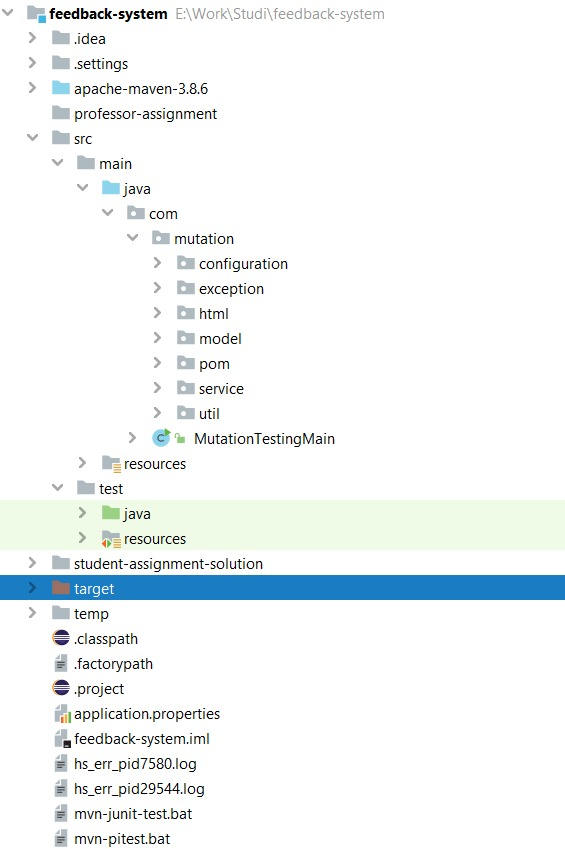
\includegraphics[width=0.60\linewidth]{content/fig2.jpg}
% 	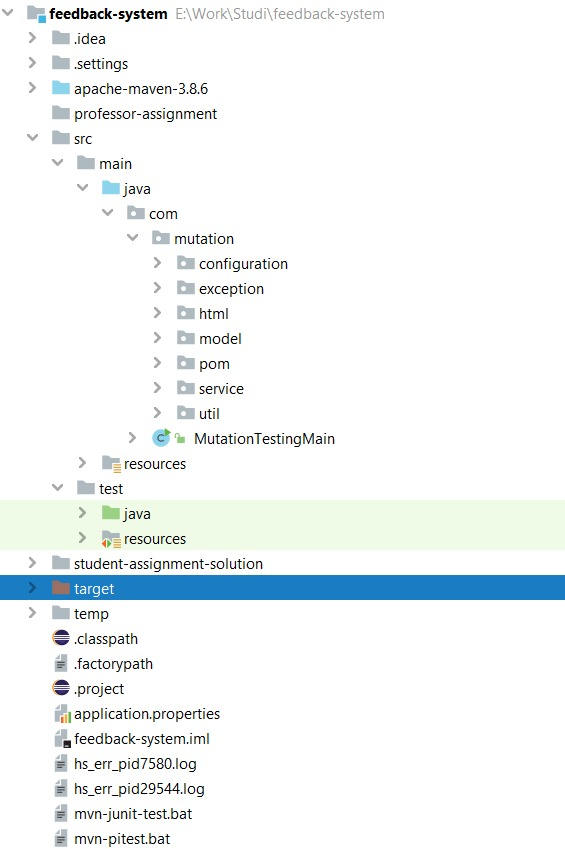
\includegraphics[scale=0.45]{content/fig2.jpg}
	\caption{Project structure}
	\label{fig:f12}
 \end{figure}

\subsection{Technologies and Tools used}
Technologies that are used in this project include:\\
intellij/eclipse sts, Java version 17, Maven, JUnit, PiTest, JSoup HTML Parser, Commons-IO, Zip4j, EclEmma, Log4j and Dropbox. \\
All the dependencies can be found in the “pom.xml” file.
\newline A Project Object Model (POM) is the core unit of Maven's build system. It is an XML document that contains information about the project, such as its configuration details, and provides default values for most projects. POMs are used by Maven to construct a project's overall build process, allowing developers to easily manage dependencies, build processes, and other aspects of the project. For the vast majority of projects, it comes with default settings.
\begin{itemize}
\item Java 17: As the newest long-term support (LTS) release for Java under its six-monthly release cycle, Java 17 is the latest release under that cycle. It was developed in collaboration with Oracle engineers as well as the entire Java community via the OpenJDK Community and the Java Community Process (JCP).
\item JUnit: As the name implies, JUnit is a framework for unit testing for the Java programming language. The JUnit framework is one of a family of unit testing frameworks that are collectively known as xUnit that originated with SUnit, and has played a very important role in the development of test-driven development. When Junit is compiled, it is linked as a JAR file and it is included in the build process.
\item PITEST: PITEST is a state-of-the-art mutation testing system that provides Java and the JVM with standard coverage for any changes made during development. This tool has a fast, scalable configuration, and it integrates well with modern tools for testing and building.
\item Mutation testing: The purpose of mutation testing is to improve the adequacy of tests and to uncover defects in a program by testing it against a range of different mutations. This is based on the idea that the production code is going to be changed dynamically and, as a result, the tests will fail.
\item Jsoup: This open-source Java library is designed to parse, extract, and manipulate data stored in HTML files.
\item Commons-IO: This is a collection of utilities for developing IO functionality as a part of Apache Commons IO. Among the six main areas in this package, there are six main groups: io - This package defines utility classes for working with streams, readers, writers, and files. File Comparator - This package provides different implementations of File Comparators for use with various file types.
\item Zip4j: This is the most complete Java library for zip files or streams. It also supports zip encryption.
\item Maven project manager tool. The Apache Group created the well-known open-source build tool Maven to create, publish, and distribute various projects simultaneously for improved project management. It is a tool that allows programmers to create and document the dynamic framework.
\item Log4j: It is a component of the Apache Software Foundation's Apache Logging Services project written by Ceki Gülcü.  
\end{itemize}

\newpage
\subsection{Architecture}
\subsubsection{Dropbox}
The feedback system uses Dropbox to store project files that have been submitted by students. Dropbox has four main folders. They include Submitted Project, the Project Success, projects processing and the Project Failure.
\begin{itemize}
\item Submitted Project: This folder contains projects that have been submitted by students.
\item Project Success: This folder contains project-passed Junit test and PiTest. Rclone moves these projects from the Local Server to the Project Failure folder.
\item Project Failure: This folder contains projects that have not passed the Junit test and PiTest. Rclone moves these projects from the Local Server to the Project Failure folder.
\item projects processing: this folder contains projects for processing.  
\end{itemize}
\subsubsection{Local Server}
This is a server where Feedback-Application is deployed and Rclone Program is installed. The Server has three parts that include: Folder directories, Rclone, and Feedback-App.
\subsubsection{Folder Directories}
The Local Server has four folder directories, which include Submitted Project, Project Processing, Project Success, and Project Failure.
\begin{itemize}
\item Submitted Project: This folder contains projects submitted by students. The projects are moved from Dropbox to the Local Server by the Rclone program. The Feedback application reads this folder to find the submitted project that needs to run the test.
\item Project Processing: After Feedback application has found the projects in the Submitted Project folder, the Feedback application then moves those projects to the Project Processing folder to perform the test. 
\item Project Success: If that project passes both the Junit and PiTest test, the project is moved to the Project Success folder.
\item Project Failure: If that project fails to pass both Junit test and PiTest, it will then moved to the Project to the failure folder.
\end{itemize}
\subsubsection{Rclone}
Rclone is a command line program to manage files on cloud storage. It is a feature-rich alternative to cloud vendors' web storage interfaces and supports over 40 cloud storage products including S3 object stores, business \& consumer file storage services, as well as standard transfer protocols. Rclone's familiar syntax includes shell pipeline support, and dry run protection. It is used at the command line, in scripts, or via its API. Rclone has been used in this feedback system to move files between the Local Server and Dropbox, ensuring anonymity. Rclone is a command line program that is used to automate the process of moving files between these two locations.\par  

Rclone does the heavy lifting of communicating with cloud storage for users to move files between Dropbox and Local Server in such a way that it maintains file integrity by checking MD5 & SHA1 hashes at all times as well as preserving timestamps of file. Scheduled events help trigger Rclone program which moves files from Dropbox: submitted project to local: submitted project; local: project success to Dropbox: project success; local: "project failure" to Dropbox: "project failure". This helps ensure that projects are moved efficiently between the two locations without any data loss.\par 

The system flow begins with a Scheduled timer event which triggers the Rclone program to execute its steps. The first step is for Rclone to move files from Dropbox: submitted project to local: submitted project. This moves the files from Dropbox into the Submitted Project folder on the Local Server. 

The second step is for Rclone to move files from local: project success to Dropbox: project success. This moves all projects that have passed both Junit test and PiTest from the Local Server into the Project Success folder on Dropbox.   

The third and final step is for Rclone to move file from local: "project failure" to Dropbox: "project failure". This moves all projects that have failed both Junit test and PiTest from the Local Server into the Project Failure folder on Dropbox. After this, the system flow will end.\par 

Rclone is mature, open-source software originally inspired by rsync and written in Go. It mounts any local, cloud or virtual filesystem as a disk on Windows, macOS, Linux and FreeBSD and also serves these over SFTP, HTTP, WebDAV, FTP and DLNA. Third-party developers create innovative backup, restore, GUI and business process solutions using the rclone command line or API.

\subsubsection{Feedback Application}
The Feedback application is designed to help students gain a better understanding of their coding assignments. It reads the submitted projects and performs Junit test and PiTest. If the project passes both tests, it is moved to the Project Success directory. However, if it fails either of the tests, it is moved to the Project failure directory.\par 
The Feedback application then generates a report that provides hints and feedback to the students regarding how they can improve their code in order to pass the PiTest. This report helps students understand what areas they need to focus on in order to be successful with their projects. \par 
The Feedback application also scans submitted projects for any folders; if found, these are moved to the Project Processing directory. From here, each project folder is tested one by one until all have been tested and processed. \par 
The Feedback application is an invaluable tool for students who may be struggling with coding projects or who just want to further hone their skills. It allows them to quickly identify issues with their code and take actionable steps toward improving it, resulting in better outcomes for their projects.
\newpage
\begin{figure}[h!]
	\centering
	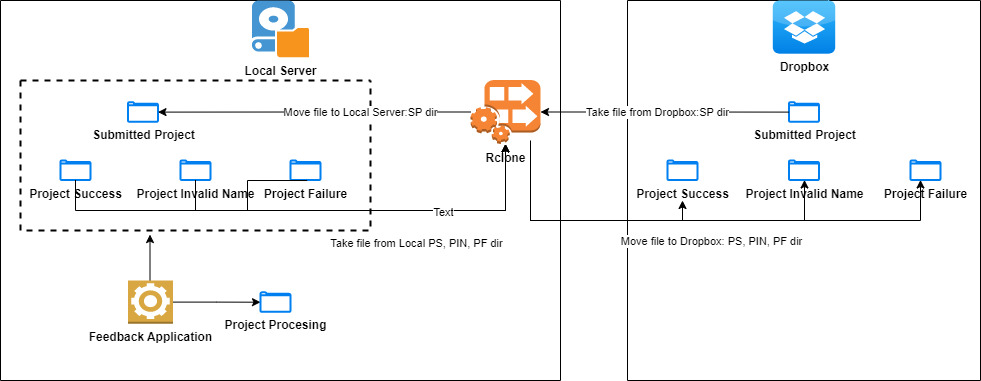
\includegraphics[scale=0.46]{content/fig3.jpg}
	\caption{Architecture}
	\label{fig:f11}
\end{figure}
\section{Service Flow}
\subsection{ Main flow}
This is the flow that shows the steps and stages that take place when a student solution is submitted to the feedback system. These steps are explained below:
\begin{itemize}
\item Scheduled: This is the section that shows a timer event start. The user in the configuration file will schedule it. Example: Run every 8 am from Mon-Fri. Whenever the timer reaches the main flow it will be triggered to start.
\item Check local: Submitted project directory. It is a stage that checks whether the submitted projects directory has a new folder or not.
\item Is have new file: This is a condition activity. It checks whether a new project has been submitted, and move to the next stage. If no new project has been submitted the system will end the process.
\item Move file to local: Project processing directory. At this stage, the project folder is moved from the submitted project to the project processing directory.
\item Execute Junit test: Here, the Junit tests from the project folder are performed one by one in the project processing directory.
\item Junit test pass: Here if the project file passes the Junit test, they proceed to the Execute PiTest stage. However, if the Junit test fail, they move to the Move file to local: project failure.
\item Move file to local: Project failure. This is where project files move when they fail to pass Junit test move. 
\item Execute PiTest: This is where PiTest is performed on project files that passed Junit test. 
\item PiTest pass: Here if the project file passes the PiTest, they proceed to the Move file to local: project passed. However, if the Junit test fail, they move to the Send email notification for the report test stage.
\item Move file to local: project success. This is the stage where the project file that passes PiTest moves the project folder from the project progressing directory to the project success directory.
\item Send email notification: This is the stage where a report is generated, then sent to the Professor and the Student who owns the project. After this, the process ends. 
\newpage
\end{itemize}
 \begin{figure}[h!]
% 	\centering
   \begin{tikzpicture}[node distance = 2cm, auto]
         %node plot
    \node[cloud](H2){Scheduled};
    \node[block,below of=H2](check){Check local sumitted project directory};
    \node[decision,below of=check](file){Is have new file?};
     \node[cloud, right of = file, node distance =4.5cm](elipsee){end no project};
    \node[block,left of = file, node distance= 4.5cm](move){Move file to local project processing folder};
    \node[block,below of=move, node distance =3.5cm](unit){Excute unit test};
     \node[decision,right of=unit, node distance =4.5cm](is unitest){Is unitest passed?};
    \node[block,below of=is unitest, node distance=2.7cm](pitest){Excute pitest};
    \node[decision,below of=pitest, node distance=2.7cm](third){Is pitest passed?};
    \node[block, right of = third, node distance =4.5cm](elipse){move file to local project failed};
    \node[block, left of = third, node distance = 4.5cm](moved){Move file to local project passed};
   \node[block, below of = moved, node distance =3cm](send){Send email notification testing result and attaches report file};
    \node[cloud, right of = send, node distance=4.6cm](final){end};
    % \node[block, below of =local pro, node distance =2.5cm](send){Send email notification testing result and attaches repr0t file};
    \path[line](H2)--(check);
    \path[line](check)--(file);
     \path[line](file)--node[near middle, color=black]{Yes}(move);
      \path[line](move)--(unit);
    \path[line](unit)--(is unitest);
     \path[line](is unitest)--node[near middle, color = black]{Yes}(pitest);
     \path[line](pitest)--(third);
     \path[line](third)--node[near middle, color = black]{Yes}(moved);
     \path[line](moved)--(send);
        \path[line](send)--(final);
        \path[line](elipse.south)|-(send.north);
        \path[line](third)--node[near middle, color=black]{No}(elipse);
       \path[line](is unitest)-|node[near middle, color=black]{No}(elipse);
       \path[line](file)--node[near middle, color=black]{No}(elipsee)
    \end{tikzpicture}
    \caption{Main Flow}
% 	\label{fig:f22}
 \end{figure}
% \begin{figure}
% 	\centering
% 	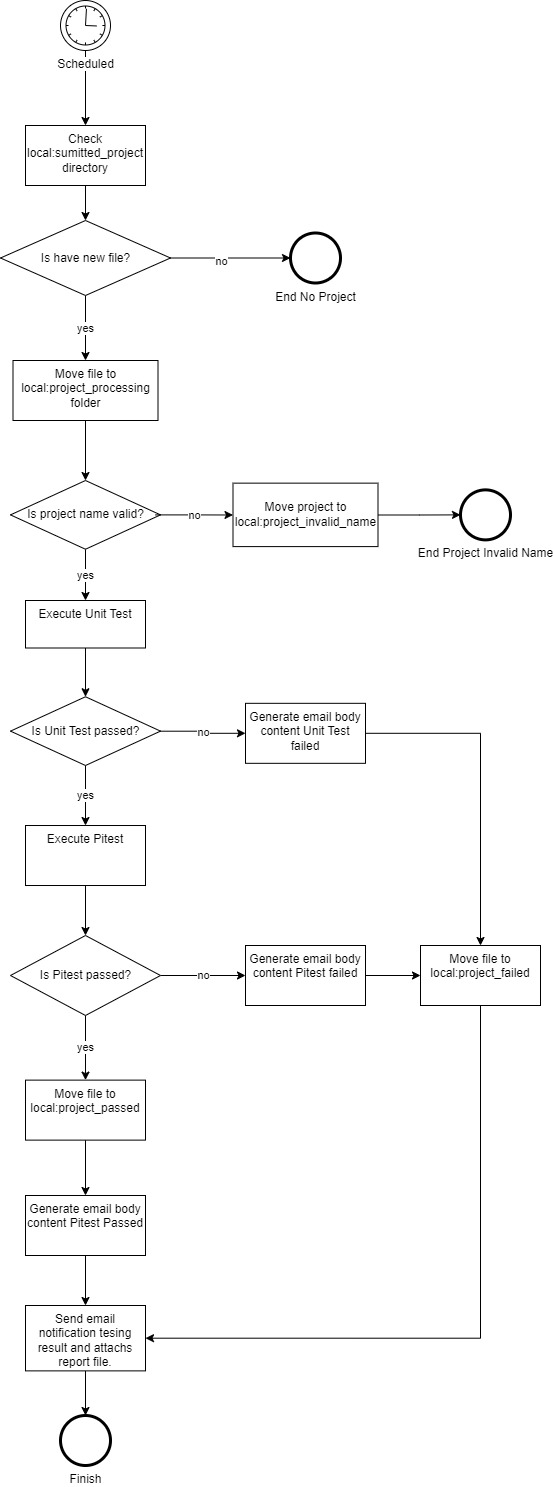
\includegraphics[width=0.45\linewidth]{fig4.jpg}
% 	\caption{Main Flow}
% 	\label{fig:f11}
% \end{figure}
\newpage
\subsection{Junit test Flow}
The Junit flow starts with the JobStartMainFlow function, which calls setupSelectedProjectTesting() method on MutationTestingService class to set up and perform unit tests and mutation tests on the project. The createCommandsForUnitTestingWithFullProjectPath() method is then called on MutationTestingService class to create commands for unit testing. 
Then, writeCommandToFile() method is called to write the command to a file called “mvn-junit-test bat”. After that, performJUnitTestingProcessBuilder() method is called to execute the unit test. If the unit test fails, it will return false, otherwise it will move to the next step of executing mutation testing. This is a flow that is triggered by the main project flow and it involves five main steps that are summarized below:
\begin{itemize}
\item Create command for Junit test: This is the stage where the command is created to run the Junit test. The command is then saved to a file type “.bat”, which is later executed by the system.
\item Perform Junit test: This is the stage where the file generated from step 1 is executed.
\item Junit test passed: Here, Junit test is performed on the files, and if they pass, they are moved to the PiTest Performing stage. However, if they fail, they are moved to the Return status failed at Junit stage.
\item Return status failed at Junit test: This is where files that have failed the JUnit test are moved to the failure directory and the Junit test flow ends. 
\item Perform PiTest flow: This is where PiTest is performed on the files that passed Junit test. 
\end{itemize}
\begin{figure}[h!]
	\centering
 \begin{tikzpicture}[node distance = 2cm, auto]
    \node[cloud](H4){unitest triggered};
    \node[block,below of=H4, node distance=3.1cm](create){Create command for unitest};
    \node[block,below of=create, node distance =3.5cm](perform){Perform unitest};
    \node[decision,below of=perform,node distance=3.5cm](passed){Is unit test passed?};
    \node[block, right of=passed,node distance=4.5cm](Return){Return status failed at unit test};
    \node[cloud, right of=Return,node distance=4.5cm](two){End};
    \node[block, below of = passed, node distance =3.2cm](return){Perform pitest};
     \path[line](H4)--(create);
     \path[line](create)--(perform);
     \path[line](perform)--(passed);
     \path[line](passed)--node[near middle,color=black]{Yes}(return);
     \path[line](return)-|(two);
     \path[line](passed)--node[near middle, color = black]{No}(Return);
     \path[line](Return)--(two);
    %  \path[line](passed)--node[near middle, color = black]{No}(low side);
    \end{tikzpicture}
    \caption{Junit Test Flow }
	\label{fig:f33}
\end{figure}\\
% \begin{figure}[h!]
% 	\centering
% 	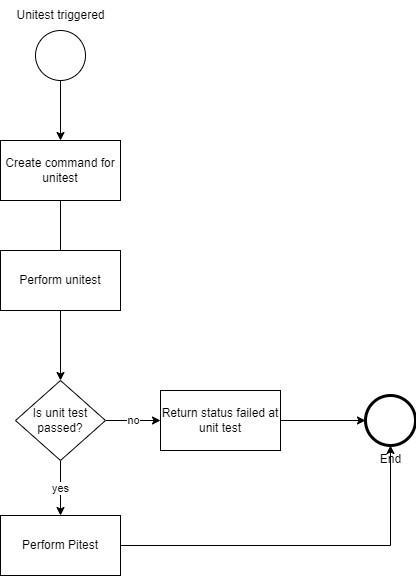
\includegraphics[scale=0.55]{fig5.jpg}
% 	\caption{Junit Test Flow }
% 	\label{fig:f11}
% \end{figure}\\
\newpage
\subsection{PiTest flow}.
The includePiTestDependencyInPomFileFullProjectPath() method is first called on MutationTestingService class to include PiTest dependency in pom.xml file. Then, writeModifiedModelToFileWithFullProjectPath() method is used to write PiTest dependency to pom.xml file in ModifyPomXml class. In ModifyPomXml class, the populateModifiedModelWithFullProjectPath() method is used to parse pom.xml file to a Model object. The addPiTestDependency() method and addPlugin() method are used to add PiTest dependency alongside with the plugin respectively in pom.xml file before returning it back to MutationTestingService class. Once it is returned, the createCommandsForMutationTestingWithFullProjectPath() method is called to create commands for mutation testing and the performMutationTestingUsingProcessBuilder() method is used to execute the mutation test before returning true if it is successful or false if unsuccessful. By following this process, students can receive feedback about their assignments in a timely manner regarding their code quality based on the results of their test suite.\\
The PiTest flow has eight main function. The flow is triggered by the main process flow.
\begin{itemize}
\item Scan pom.xml file: This is the first stage of the PiTest flow where the project folder is scanned to read the content of “pom.xml” file.
\item Is PiTest dependency Injected: Here, the “pom.xml” file is checked to see if it has PiTest dependency. If PiTest dependency is present it will proceed to Create the command for PiTest stage. However, if the PiTest dependency is not present it moves to the Inject PiTest dependency stage.
\item Inject PiTest dependency: Here, the PiTest dependency is added to the “pom.xml” file.
\item Create Command for PiTest: This is the stage where the command is created to run the PiTest. The file is saved to a file type “.bat”.
\item Perform PiTest. This is where the PiTest is performed on the test suite generated from the Create Command for PiTest.
\item Is PiTest pass: Here, if the test suite pass the PiTest stage, they proceed to the Return status success at PiTest. However, if the test suite fail PiTest, they are moved to the Return status failed at PiTest.
\item Return status failed at PiTest: Here, the status of the test suite that failed to pass PiTest is displayed and then the process ends.
\item Return status success at PiTest: Here, the status of the test suite that passed PiTest will be displayed and then the process ends.
\end{itemize}
 \begin{figure}[h!]
	\centering
\begin{tikzpicture}[node distance = 2cm, auto]
    %node plot
    \node[cloud](H1){pitest trigered};
    \node[block,below of=H1, node distance=2cm](scan){Scan pom.xml file};
    \node[decision,below of=scan](pitest){Is pitest dependency rejected?};
    \node[block,right of = pitest, node distance= 4.5cm](inject){Inject pitest dependency};
    \node[block,below of=pitest, node distance =3.1cm](creat){create command for pitest};
    \node[block,below of=creat](perform){Perform pitest};
    \node[decision, below of = perform](passed){Is pitset passed?};
    \node[block, right of =passed, node distance =4.5cm](low side){return status failed at pitest};
    \node[cloud, right of =low side, node distance 2cm](two side){end};
    \node[block, below of = passed, node distance =2.7cm](return){return status successed at pitest};
    \path[line](H1)--(scan);
    \path[line](scan)--(pitest);
    \path[line](pitest)--node[near middle, color=black]{Yes}(creat);
    \path[line](creat)--(perform);
    \path[line](perform)--(passed);
    \path[line](passed)--node[near middle, color = black]{Yes}(return);
    \path[line](pitest)--node[near middle, color = black]{No}(inject);
     \path[line](passed)--node[near middle, color = black]{No}(low side);
      \path[line](low side)--node[near middle, color = black]{No}(two side);
        \path[line](return)-|(two side);
        \path[line](inject)|-(perform);
    \end{tikzpicture}
    	\caption{PiTest Flow}
	\label{fig:f11}
\end{figure}
% \begin{figure}
% 	\centering
% 	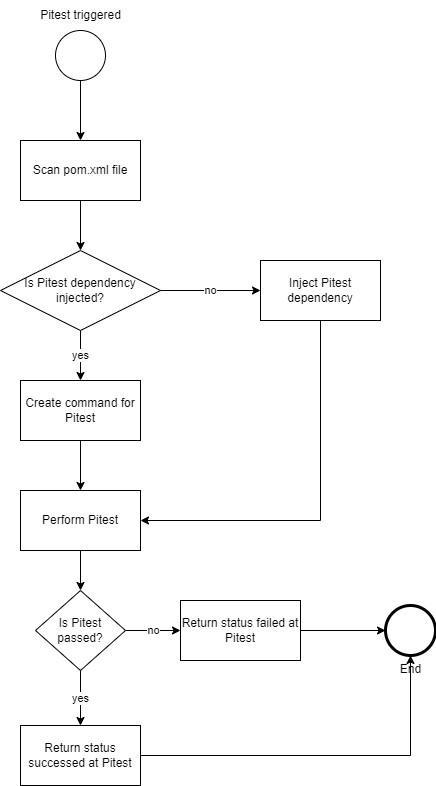
\includegraphics[scale=0.70]{fig6.jpg}
% 	\caption{PiTest Flow}
% 	\label{fig:f11}
% \end{figure}

\newpage
\subsection{Moving File Flow}
\begin{itemize}
\item Scheduled: This timer event starter is configured to trigger the Rclone program.
\item Rclone move files from Dropbox: Move submitted project to local submitted project directory. Rclone moves the file submitted project directory from Dropbox to the Local Server in the submitted project directory.
\item Rclone move files from local: Move project success to Dropbox project success directory. Rclone moves the file project success directory from Dropbox to the Local Server in the project success directory.
\item Rclone move files from local: Move project failure to Dropbox project failure directory. Rclone moves the file project failure directory from Dropbox to the Local Server in the project failure directory. After this the system flow will end
\end{itemize}
\begin{figure}[h!]
	\centering
 \begin{tikzpicture}[node distance = 2cm, auto]
    \node[cloud](H3){Scheduled};
    \node[block,below of=H3, node distance=3.1cm](Rclone){Rclone move file from Dropbox submitted project to local submitted project};
    \node[block,below of=Rclone, node distance =3.5cm](failed){Rclone move file from local project failed to Dropbox project failed};
    \node[block,below of=failed,node distance=3.5cm](success){Rclone move file from local project success to Dropbox project success};
    \node[cloud, below of = success, node distance =2.7cm](return){end};
     \path[line](H3)--(Rclone);
    \path[line](Rclone)--(failed);
     \path[line](failed)--(success);
    \path[line](success)--(return);
    % \path[line](perform)--(passed);
    % \path[line](passed)--node[near middle, color = black]{Yes}(return);
    % \path[line](pitest)--node[near middle, color = black]{No}(inject);
    %  \path[line](passed)--node[near middle, color = black]{No}(low side);
    %   \path[line](low side)--node[near middle, color = black]{No}(two side);
    %     \path[line](return)-|(two side);
    %     \path[line](inject)|-(perform);
    \end{tikzpicture}
    \caption{Moving Flow}
	\label{fig:f14}
 \end{figure}
% \begin{figure}[h!]
% 	\centering
% 	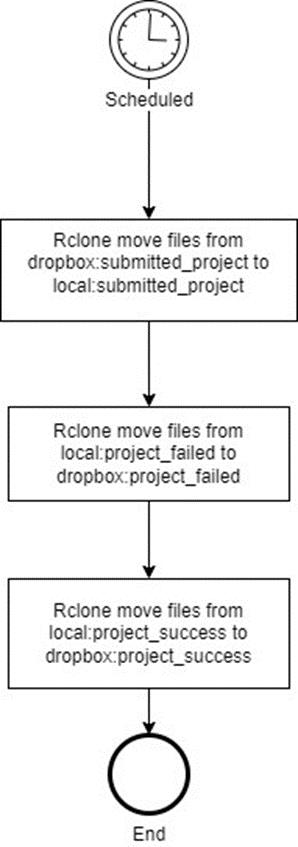
\includegraphics[scale=0.55]{fig7.jpg}
% 	\caption{Moving Flow}
% 	\label{fig:f11}
% \end{figure}
\newpage
\section{Project Diagram}
This use case diagram below give a sense of orientation of the feedback system. It provides detailed insight into the structure of the system. At the same time it offers a quick overview of the functions happening in the system as well as the two actors involved. 
\subsection{Use case diagram}

\begin{figure}[h!]
    \centering
    
    
    %\label{fig:my_label}

\begin{tikzpicture}
%big rectangle
\draw (0,0) rectangle (8,15.5);

%circles
\draw (4,13.5) ellipse (2cm and 1cm);
\draw (4,11.5) ellipse (2cm and 1cm);
\draw (4,9.5) ellipse (2cm and 1cm);
%\draw (5,10.5) ellipse (2cm and 1cm);

\draw (4,7.5) ellipse (2cm and 1cm);
\draw (4,5.5) ellipse (2cm and 1cm);
\draw (4,3.5) ellipse (2cm and 1cm);
\draw (4,1.5) ellipse (2cm and 1cm);

%rectangle text
\draw (4,15) node {Feedback System};

%circle text
\draw (4,13.5) node {Submit Project};
\draw (4,11.5) node  {View the testing results};
\draw (4,9.5) node {Receive Notifications};


\draw (4,7.5) node {Config time schedule};
\draw (4,7) node  {execute system};
\draw (4,5.5) node {Customize feedback};
\draw (4,5.) node {hint message};
\draw (4,3.5) node {Customize email};
\draw (4,3) node {content};
\draw (4,1.5) node {Config mutation};
\draw (4,1) node {threshold point};

%student arrows
\draw[arrows=->] (-2,14) -- (2,14); 
\draw[arrows=->] (-2,14) -- (2,12); 
\draw[arrows=->] (-2,14) -- (2,10); 

% student arms
\draw[black, thick] (-2,14.5) -- (-2,13);
\draw[black, thick] (-2,13) -- (-3,12);
\draw[black, thick] (-2,13) -- (-1,12);
\draw[black, thick] (-2,14) -- (-3,14);

%student head
\draw[color=black] (-2,15) circle (0.5cm);

\draw (-2,11.5) node {Students};

%professor arms 
\draw[black, thick] (11,1.5) -- (11,2.5);
\draw[black, thick] (11,2) -- (12,2);

%professor feet
\draw[black, thick] (11,1.5) -- (12,1);
\draw[black, thick] (11,1.5) -- (10,1);
%\draw[black, thick] (15,1.5) -- (14,2.5);

%professor head
\draw[color=black] (11,3) circle (0.5cm);

\draw (11,0.5) node {Professor};

\draw[arrows=->] (11,2) -- (6,7); 
\draw[arrows=->] (11,2) -- (6,5); 
\draw[arrows=->] (11,2) -- (6,3); 
\draw[arrows=->] (11,2) -- (6,1);


\end{tikzpicture}
\caption{Use Case Diagram}
\label{fig:f11}
\end{figure}

% \begin{figure}[h!]
% 	\centering
% 	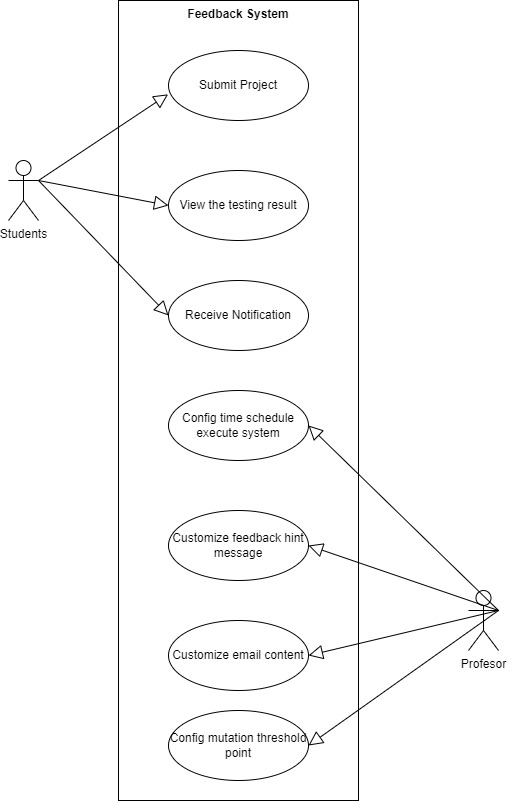
\includegraphics[scale=0.45]{fig8.jpg}
% 	\caption{Class Diagram}
% 	\label{fig:f11}
% \end{figure}


\subsubsection{Mutation Testing Main class}
The Main class of this application will be executed first when the application executes.
\subsubsection{Properties Configuration class}
This class is used for initial configuration for the whole project. The static factory constructor from application Properties file() loads configuration from the "application.properties" file, then sets it to an instance of the Properties Configuration object.
\begin{figure}[h!]
	\centering
	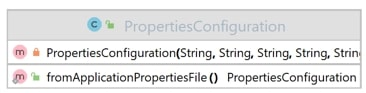
\includegraphics[scale=0.90]{content/fig9.jpg}
	\caption{Properties Configuration class}
	\label{fig:f11}
\end{figure}
\subsubsection{Job Start MainFlow class}
This class is implemented from Job class, which belongs to Quartz dependency. JobStartMainFlow class is a presentation of the main flow diagram.
\begin{figure}[hb]
	\centering
	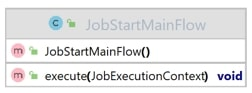
\includegraphics[scale=0.90]{content/fig10.jpg}
	\caption{Job Start Main Flow class}
	\label{fig:f11}
\end{figure}

Dependencies:
\begin{itemize}
 \item ProjectDirServiceImpl.class
\item Email ServiceImpl.class
\item Mutation Testing Service.class
\item Html Reader.class
\end{itemize}
\subsection{Project DirServiceImpl class}
This class is implemented from ProjectDirService class which provides service related to ProjectDir(submitted project dir, processing project dir, failure project dir and success project dir).
\begin{figure}[h!]
	\centering
	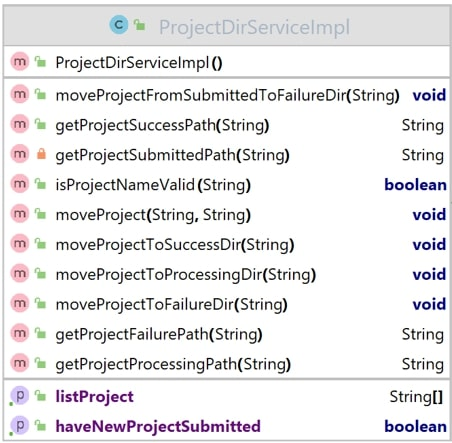
\includegraphics[scale=0.70]{content/fig11.jpg}
	\caption{Project DirServiceImpl class}
	\label{fig:f11}
\end{figure}
\newpage
Dependencies:
\begin{itemize}
\item Properties Configuration.class
\item Project DirService.class
\end{itemize}
\subsubsection{Email ServiceImpl class}
This class is implemented from Email Service class. This class provides service related to email actions such as send Email(), send Email With Attachments().\\
\begin{figure}[h!]
	\centering
	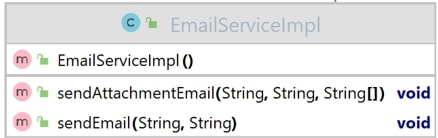
\includegraphics[scale=0.80]{content/fig12.jpg}
	\caption{Email ServiceImpl class}
	\label{fig:f11}
\end{figure}\\
\newpage
Dependencies:
\begin{itemize}
\item Email Service.class
\end{itemize}
\subsubsection{Mutation Testing Service.class}
This class is used for setting up and performing Junit test as well as PiTest.\\
By setting up I mean verifying the pom.xml file and injecting PiTest dependency in cases that it is not injected.
\begin{figure}[h!]
	\centering
	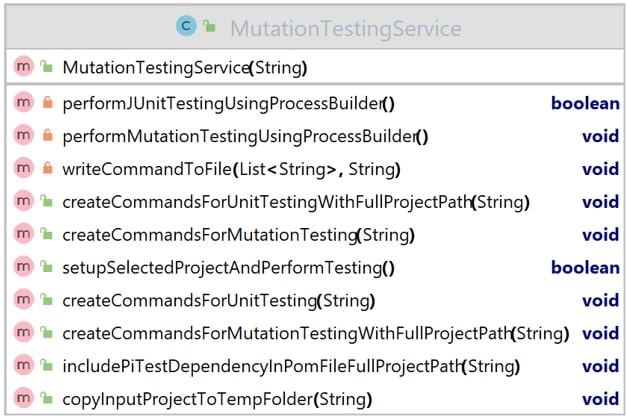
\includegraphics[scale=0.70]{content/fig13.jpg}
	\caption{Mutation TestingService class}
	\label{fig:f11}
\end{figure}\\
Dependencies:
\begin{itemize}
\item Modify PomXml.class
\item ProjectDirServiceImpl.class
\end{itemize}
\subsubsection{HtmlReader class}
The HtmlReader class is used to read the .html files generated by the PiTest mutation testing tool, extract the results, and write them to a file called "feedBackReport.txt" which can then be sent in an email.
\begin{figure}
	\centering
	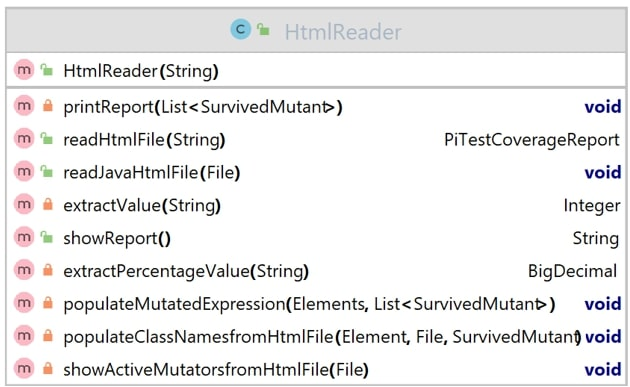
\includegraphics[scale=0.70]{content/fig14.jpg}
	\caption{HtmlReader class}
	\label{fig:f11}
\end{figure}
\newpage
Dependencies:
\begin{itemize}
\item Mutation Sample Message Service.class
\item ProjectDirServiceImpl.class
\item PiTest Coverage Report.class
\item Feed back Message Service.class
\end{itemize}
\subsubsection{ProjectDirService class}
This is an interface that defines the methods for the ProjectDir object.
\begin{figure}[h!]
	\centering
	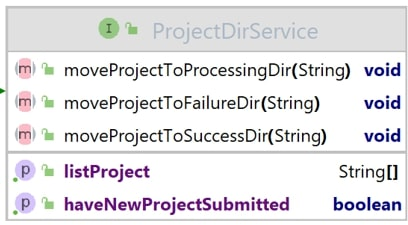
\includegraphics[scale=0.65]{content/fig15.jpg}
	\caption{Project DirService Interface}
	\label{fig:f11}
\end{figure}
\subsubsection{Email Service class}
This is an interface that defines the methods for the Email object.
\subsubsection{Modify PomXml.class}
This class is used to read the pom.xml file in submitted project, add PiTest dependency and PiTest plugin to that pom.xml file.\\
\\
Dependencies:
\begin{itemize}
\item InvalidProjectExeption.class
\item ProjectDirServiceImpl.class
\end{itemize}
\begin{figure}[h!]
	\centering
	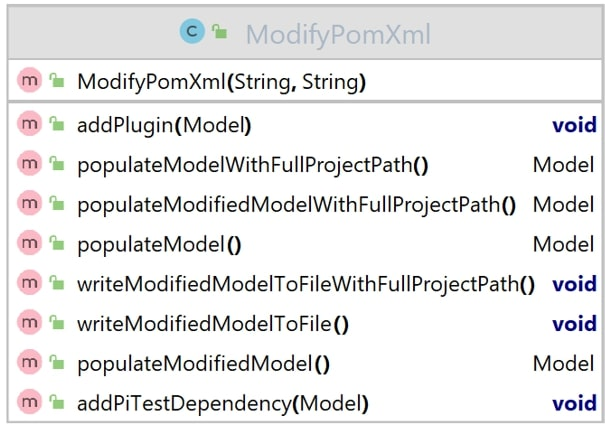
\includegraphics[scale=0.70]{content/fig16.jpg}
	\caption{Modify PomXml class}
	\label{fig:f11}
\end{figure}

\subsubsection{Mutation Sample Message Service class}
This class loads the samples of mutation and the solution for each mutation operator. These files contain samples located in the “src/main/resources” directory.
\newpage
\begin{figure}[h!]
	\centering
	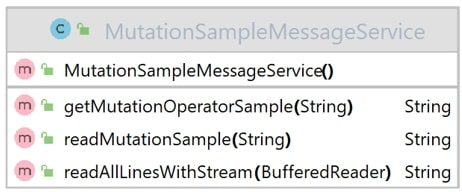
\includegraphics[scale=0.80]{content/fig17.jpg}
	\caption{Mutation Sample Message Service class}
	\label{fig:f11}
\end{figure}

\newpage
\begin{figure}[h!]
	\centering
	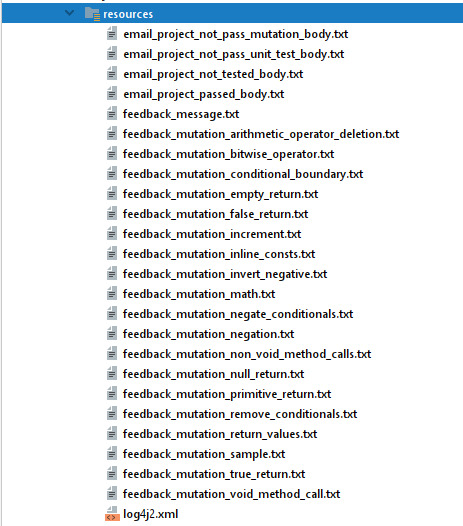
\includegraphics[scale=1.8]{content/fig18.jpg}
	\caption{Mutation Samples File}
	\label{fig:f11}
\end{figure}
\subsubsection{PiTest Coverage Report class}
This is the model class that presents PiTest coverage report object.
\newpage
\begin{figure}[h!]
	\centering
	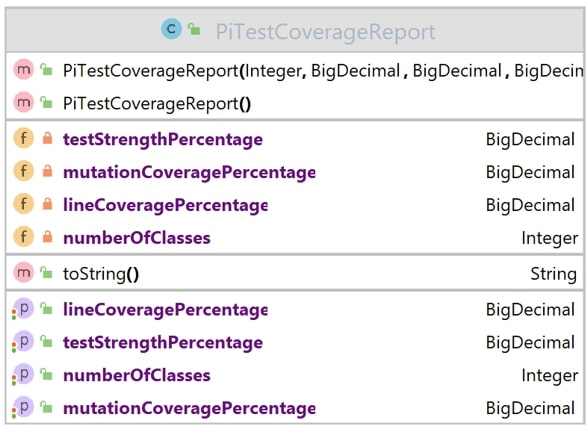
\includegraphics[scale=0.70]{content/fig19.jpg}
	\caption{PiTest Coverage Report class model}
	\label{fig:f11}
\end{figure}

\subsubsection{Feedback Message Service class}
This class reads the file “feedback message.txt” from the “src/main/resources” directory then generates a feedback message base on the mutation result.
\newpage
\begin{figure}[h!]
	\centering
	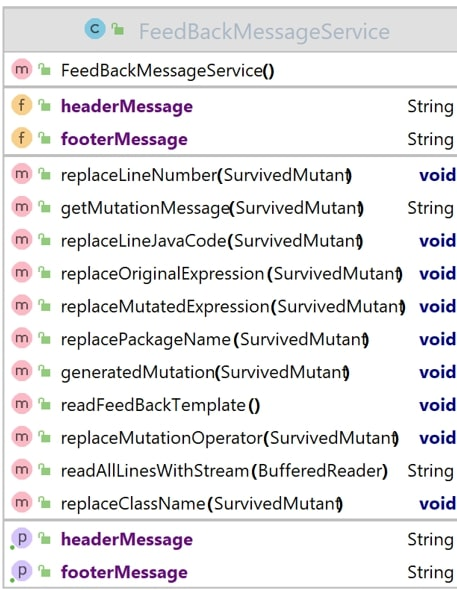
\includegraphics[scale=0.70]{content/fig20.jpg}
	\caption{Feedback Message Service class}
	\label{fig:f11}
\end{figure}
\subsubsection{Invalid Project Exeption class}
This is a custom exception handler model.
\newpage
\begin{figure}[h!]
	\centering
	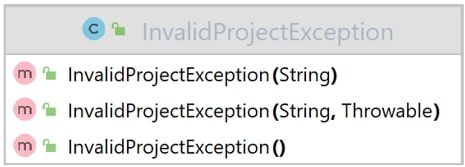
\includegraphics[scale=0.70]{content/fig21.jpg}
	\caption{Invalid Project Exception class}
	\label{fig:f11}
\end{figure}
\subsubsection{Survived Model class}
This is the model present for Survived Mutation object when executing PiTest
\begin{figure}[h!]
	\centering
	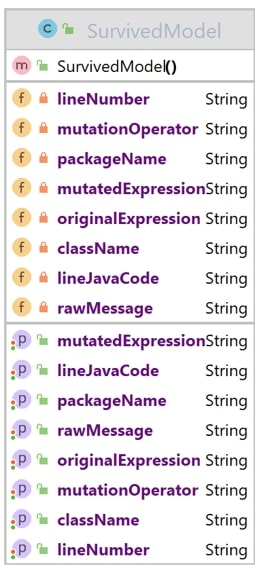
\includegraphics[width=0.40\linewidth]{content/fig22.jpg}
	\caption{Survived Model}
	\label{fig:f11}
\end{figure}

\subsubsection{FeedBack Template Parameter class}
This class declares configuration parameter mapping for the feedback file in “src/main/resources/feedback message.txt”
\begin{figure}[h!]
	\centering
	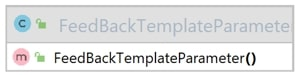
\includegraphics[scale=1.4]{content/fig23.jpg}
	\caption{Feedback Template Parameter}
	\label{fig:f11}
\end{figure}
%\newpage
\subsubsection{Mutation SamplesParamter.class}
This class declares configuration parameter mapping for mutation samples file in “src/main/resources/feedback mutation operatorName.txt”
\begin{figure}[h!]
	\centering
	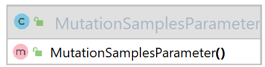
\includegraphics[scale=2.6]{content/fig45.png}
	\caption{Mutation Samples Parameter}
	\label{fig:f45}
\end{figure}

\subsection{Sequence diagram}
\subsubsection{Main Sequence Diagram}
The flow diagram that illustrates the steps and stages that must be followed in order for a solution to be submitted to the feedback system.\par 
% \begin{figure}[h!]
% 	\centering
% 	\includegraphics[scale=0.25]{content/fig24.jpg}
% 	\caption{Main sequence diagram}
% 	\label{fig:f11}
% \end{figure}
The above flow diagram illustrates the main functionalities of the Mutation Testing System. The Main class of this application will be executed first when the application executes. It starts with the Main function which trigger a scheduler, as well as loading cron expressions from an application properties file. The scheduler then invokes the Job Start MainFlow function.\par 
The Job Start MainFlow function first calls IsHaveNewProjectSubmitted() method on the Project DirServicelmpl class to check whether there are any new projects in the ‘submitted project’ folder. If there are no new projects, it will console log a description and wait for the next scheduled time. Otherwise, it will call getListProject() method on Project DirServicelmpl class to get an array of project names. \par 
It will then loop through these project names and check if each project name is invalid or not. If it is found to be invalid, it will call move Project From Submitted ToFailureDir() method on Project DirServicelmpl class to move this project from the submitted directory to a failure directory. Otherwise, it will call setup Selected Project And Perform Testing() on Mutation Testing Service to set up and perform unit tests and PiTest on the project before receiving a response if the test has been completed successfully or not from Mutation Testing Service class. \par 
If it has been completed successfully, Job Start MainFlow will call show Report() method on HtmlReader class to read the mutation testing results before sending an email notification about the results of these tests via send Email() method on Email Servicelmpl class. 

Finally, depending on whether or not the mutation testing is passed, JobStartMainFlow method will either call move Project To SuccessDir() method or move Project ToFailureDir() method on Project DirSErvicelmpl class before looping through any remaining projects in its array until all have been tested.

\subsubsection{Junit test Sequence Diagram}
In the main flow diagram, mutation testing service sets up and performs unit tests and PiTest on the project before receiving a response if the test has been completed successfully or not
\par
There are five steps that are followed in order to complete the process of Junit test which are triggered by the main flow that is shown in the flow diagram below.\par 
% \begin{figure}[h!]
% 	\centering
% 	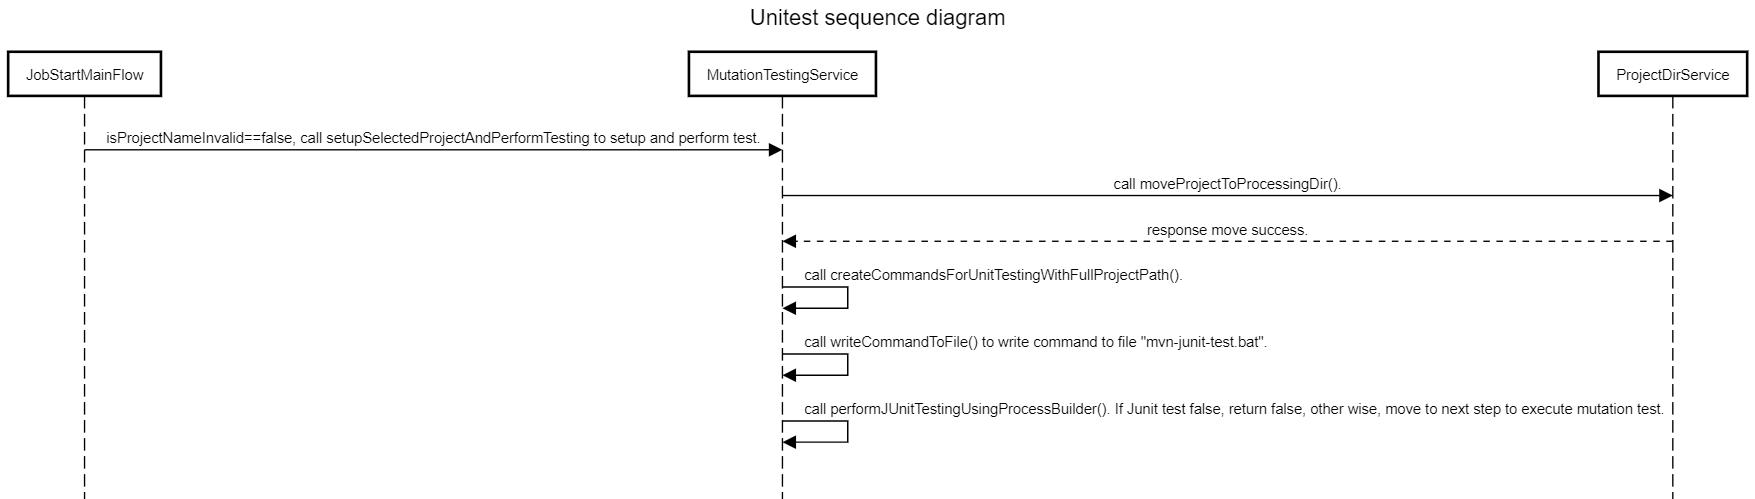
\includegraphics[scale=0.35]{content/fig25.jpg}
% 	\caption{Junit test sequence diagram}
% 	\label{fig:f11}
% \end{figure}
The above Junit test and PiTest flow starts with the Job StartMainFlow function, which calls setupSelected Project Testing() method on Mutation Testing Service class to set up and perform unit tests and mutation tests on the project. This process begins by calling create Commands For Unit Testing With full ProjectPath() method on Mutation Testing Service class to create commands for unit testing. Then, the write CommandToFile() method is called to write the command to a file. After that, perform JUnitTesting Process Builder() method is called to execute the unit test. If the unit test fails, it will return false, otherwise it will move to the next step of executing mutation test.

\subsubsection{PiTest Sequence Diagram}
This diagram shows where you can find the auto generated PiTest feedback report.\par 
% \begin{figure}[h!]
% 	\centering
% 	\includegraphics[scale=0.45]{content/fig26.jpg}
% 	\caption{PiTest sequence diagram}
% 	\label{fig:f11}
% \end{figure}
The MutationTestingService provides a way for students to obtain feedback on their code quality in a timely manner. This is achieved by first including the PiTest dependency in the pom.xml file of the project. In order to do this, the ModifiedModelToFileWithFullProjectPath() method is used to write the PiTest dependency into the pom.xml file in ModifyPomXml.PopulateModifiedModelWithFullProjectPath() method then parses the pom.xml file into a model object and adds both the PiTestDependency() and Plugin(). These are then returned back to MutationTestingService class for further processing.\par 

Once returned, createCommandsForMutationTestingWithFullProjectPath() method is called to create commands for mutation testing and perform mutation testing using ProcessBuilder() method to execute the mutation test before returning true if successful and false if unsuccessful. Through this process, students can receive feedback on their projects based on the results of these tests and make necessary changes accordingly in order to improve their code quality.
\begin{figure}[h!]
	\centering
	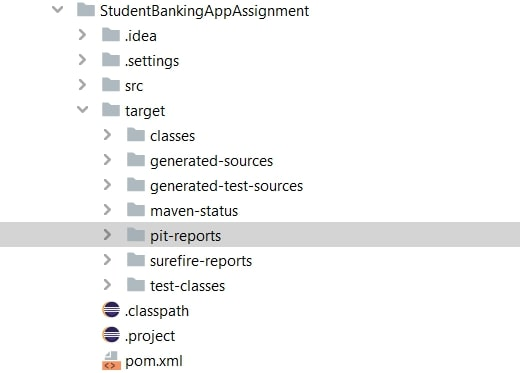
\includegraphics[scale=0.8]{content/fig27.jpg}
	\caption{PiTest report}
	\label{fig:f11}
\end{figure}
\newpage
\subsubsection{Extract report flow}
  [As discussed in the MAIN FLOW DIAGRAM, if the response has been completed successfully, Job Start Main Flow will call show Report() on Html Reader to read the mutation testing results.] \\
% \begin{figure}[h!]
% 	\centering
% 	\includegraphics[scale=0.45]{content/fig28.jpg}
% 	\caption{Extract report}
% 	\label{fig:f11}
% \end{figure}
% \newpage
The extract report flow begins with the JobStartMainFlow function, which calls ShowReport() method on HtmlReader to read the mutation testing results. After reading the HTML files, HtmlReader extracts the report and stores it in the PiTestCoverageReport model. It also reads and prints the report details to a file named “feedbackReport.txt”.\par
The response of the testing is then sent back to JobStartMainFlow. Subsequently, JobStartMainFlow triggers an email notification about the results of these tests through SendAttachmentEmail() method, attaching the “feedbackReport.txt” file to EmailServicelmpl class.\par 
Depending on whether or not the mutation testing passed, JobStartMainFlow will either call moveProjectToFailureDir() method on EmailServicelmpl class or moveProjectToSuccessDir() method on ProjectDirServicelmpl class before looping through any remaining projects in its array until all of them have been tested. This ensures that students receive accurate feedback about their projects in a timely manner.
\subsubsection{Unit test cases}
JUnit library is used to create unit test cases. Three test classes were added to cover unit testing of all logic parts in the application. These three classes are available in the package com.mutation.service under the folder src/test/java.
\subsection{Maven library}
Maven library added to the application is to execute JUnit testing and PiTesting of the submitted project.
%\newpage
\begin{figure}[h!]
	\centering
	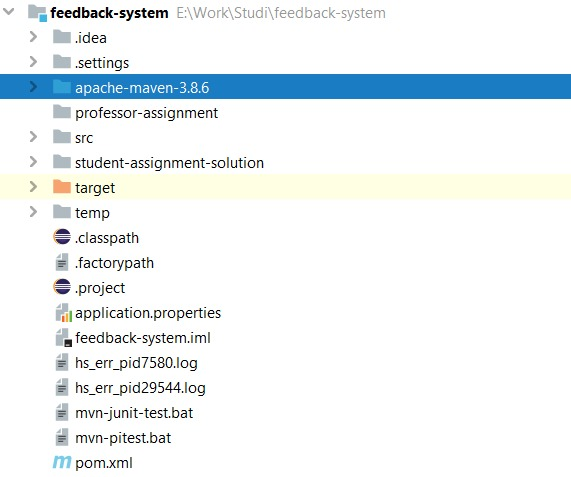
\includegraphics[scale=0.70]{content/fig29.jpg}
	\caption{maven library}
	\label{fig:f11}
\end{figure}
\subsection{Folders}
\subsubsection{Submitted Folder}
This is a local folder, which store student submitted projects. This project synced with the Dropbox submitted projects folder.\\
The dir path config in application.properties files.
\begin{figure}[h!]
	\centering
	
\includegraphics[scale=0.52]{content/fig30.jpg}
	\caption{Submitted folder configuration}
	\label{fig:f11}
\end{figure}
\newpage
\subsubsection{Project Processing}
This is a local folder that stores student projects while they are being tested. The dir path config in application.properties files.
\begin{figure}[h!]
	\centering
	
\includegraphics[scale=0.52]{content/fig31.jpg}
	\caption{Project Processing folder configuration}
	\label{fig:f11}
\end{figure}
\subsubsection{Project Success}
This is a local folder that stores student projects that are tested and pass both the Junit test and PiTest coverage threshold.\\
The dir path config in application.properties files.
\begin{figure}[h!]
	\centering
	
\includegraphics[scale=0.52]{content/fig32.jpg}
	\caption{Project Success folder configuration}
	\label{fig:f11}
\end{figure}
\subsubsection{Project Failure}
This is a local folder that stores student projects that are tested and do not pass the Junit test or PiTest coverage threshold.\\
The dir path config in application.properties files.
 \begin{figure}[h!]
	\centering
	
\includegraphics[scale=0.91]{content/fig33.png}
	\caption{Project Failure folder configuration}
	\label{fig:f11}
\end{figure}

\subsection{Application properties file}
Application.properties file is added in the project where the professor can set the threshold value of mutation coverage percentage.
\newpage
\begin{figure}[h!]
	\centering
	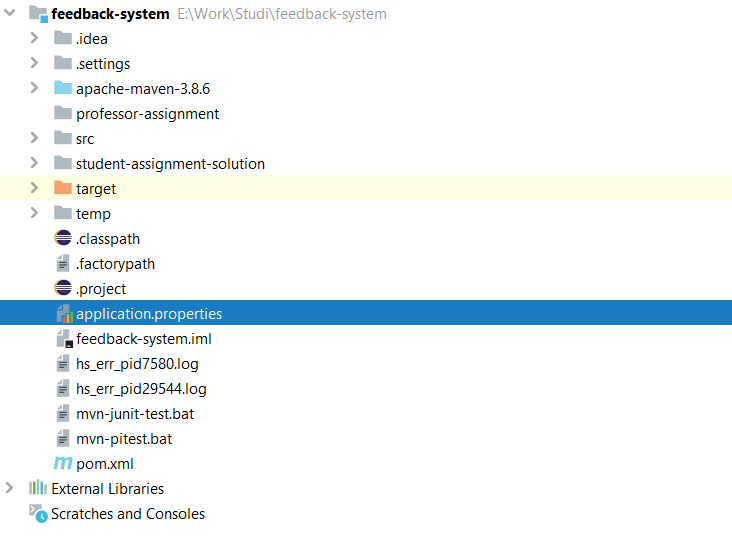
\includegraphics[scale=1]{fig34.png}
	\caption{Application properties file}
	\label{fig:f11}
\end{figure}
\subsection{Resources}
\subsubsection{Feedback message.txt.}
A template for a feedback message is found in the file feedback message.txt, which is kept in the resources folder. Using this template, a unique feedback message regarding the PiTest report's survivor mutants is created and delivered to the student as part of their feedback report.
\begin{figure}[h!]
	\centering
	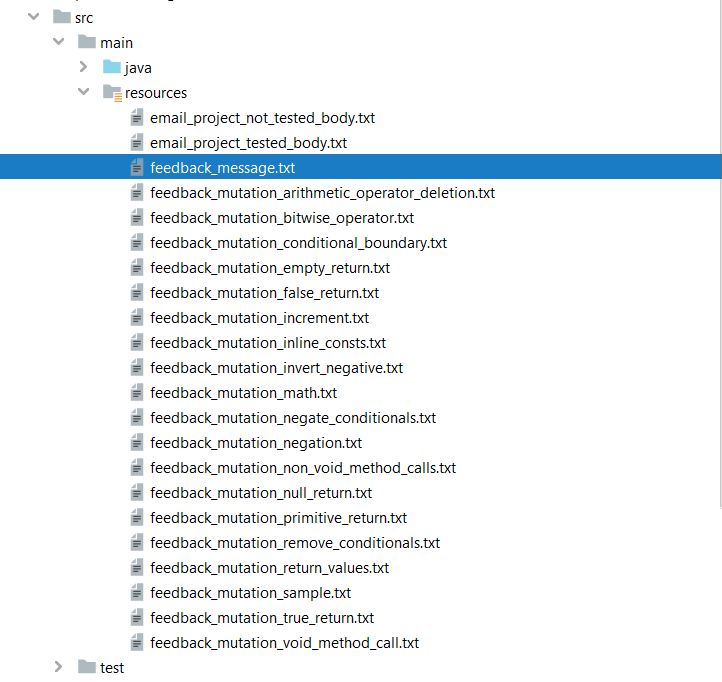
\includegraphics[scale=1]{fig35.png}
	\caption{Feedback Message file}
	\label{fig:f11}
\end{figure}
\newpage
\subsubsection{Feedback mutation sample.txt.}
The feedback mutation sample.txt file is also included in the resources folder.
\begin{figure}[h!]
	\centering
	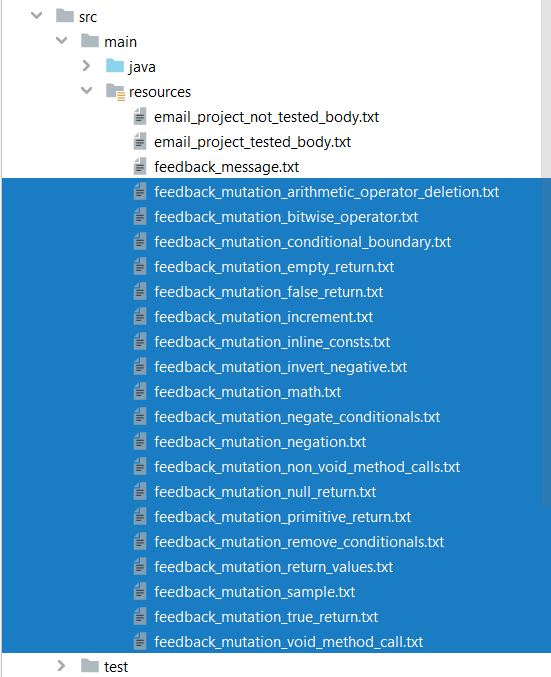
\includegraphics[scale=1.3]{fig36.png}
	\caption{Mutation Samples file}
	\label{fig:f11}
\end{figure}
\newpage
\subsection{Email project tested body.txt}
The body of email notification to students when the submitted project is tested could be a failure or success to pass the testing threshold.
\begin{figure}[h!]
	\centering
	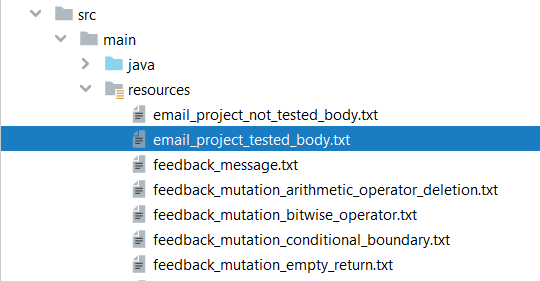
\includegraphics[scale=1.3]{fig37.png}
	\caption{Email project tested body}
	\label{fig:f11}
\end{figure}

\newpage
\subsubsection{Email project not tested body.txt}
The body of email notification to students when the submitted project is not tested could be the wrong project format name, or the project does not have a pom.xml file.\\


Dear <StudentName>\\
I am pleased to inform you that your project has been tested. Depending on the results of the testing, I have the following feedback for you:\\

\textbf{Body 1$:$ Project Not Tested$:$} The project had been scanned; however, it was not tested due to <the reason>. Please check the project in the folder 'project\_not\_tested' on Dropbox and resubmit it after you have fixed any issues. \\
\newpage
\begin{figure}[h!]
	\centering
	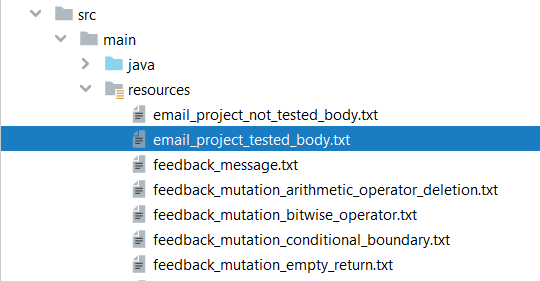
\includegraphics[scale=1.3]{fig37.png}
	\caption{Email project\_tested\_body.txt}
	\label{fig:f11}
\end{figure}\\
\textbf{Body 2$:$ Project Tested but Failed at Unit Testing$:$} The project had been scanned and tested but there are some test cases that failed. <List test case failed>. Please update these test cases and resubmit them. \\
\begin{figure}[h!]
	\centering
	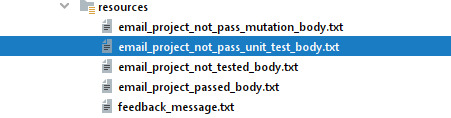
\includegraphics[scale=1.9]{content/Figure-3.34_new_-Email-project-not-pass-unit-test-body.jpg}
	\caption{Email project\_not\_pass\_unit\_test\_body.txt}
	\label{fig:f11}
 %Email project tested body
\end{figure}\\
\textbf{Body 3$:$ Project Tested but Failed at Mutation Testing$:$} The project had been scanned and tested but the test case is not good enough. You need to improve the test case to make it better. Please read the attached file 'feedBackReport.txt' for further details regarding how to improve the test case.\\
\begin{figure}[h!]
	\centering
	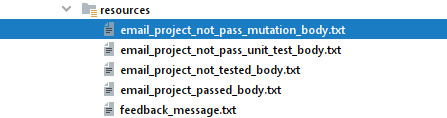
\includegraphics[scale=1.9]{content/Figure-3.35_new_-Email-project-not-pass-mutation-body.jpg}
	\caption{Email project\_not\_pass\_mutation\_body.txt}
	\label{fig:f11}
\end{figure}\\
\newpage
\textbf{Body 4$:$ Project Tested and Successful$:$} Congratulations! The project has passed all checks and been successfully tested. Well done and keep up the good work!\\
If you have any questions or would like further clarification, please do not hesitate to contact me directly or via email. \\
\begin{figure}[h!]
	\centering
	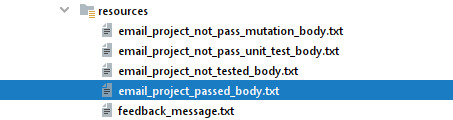
\includegraphics[scale= 1.9]{content/Figure-3.36_new_-Email-project-passed-body.jpg}
	\caption{Email project\_passed\_body.txt}
	\label{fig:f11}
\end{figure}\\
Regards,\\
$[$Professor Email Signature$]$ \\ 


\newpage
Project format name: \\ 
Mr.StudenName\_ProjectName\_Email\_yyymmddHHMM\\
Mrs.StudenName\_ProjectName\_Email\_yyymmddHHMM
%Mr.StudenName_ProjectName_Email_yyymmddHHMM 
%Mrs.StudenName_ProjectName_Email_yyymmddHHMM
\newline

Project name Restriction: \\ 
The length of the project name is can be only between 1 to 40 characters\\
\newline
Example of project name: 
%\\Mr.studiName_BankingApplicationSystem_anhnd6893@gmail.com_202301091803
\\Mr.studiName\_BankingApplicationSystem\_anhnd6893@gmail.com\_202301091803
%\newline
%   \begin{figure}[h!]
% 	\centering
% 	
\includegraphics[scale=1.1]{content/Figure-3.30_new_-Project-Invalid-Name-config.jpg}
% 	\caption{Projects\_invalid\_name}
% 	\label{fig:f11}
% \end{figure}
\subsection{Feedback report}
\subsubsection{PiTest generated report}
After executing the PiTest, the mutation test report named “PiTest-reports” will be generated in the folder name “target” of the project being tested.\par 
Example: \\%StudentBankingAppAssignment_kontaktlourenz@yahoo.de_202301070608\target\PiTest-reports
StudentBankingAppAssignment\_kontaktlourenz@yahoo.de\_202301070608\textbackslash{}target\textbackslash{}PiTest-reports
%\newpage
\begin{figure}[h!]
	\centering
	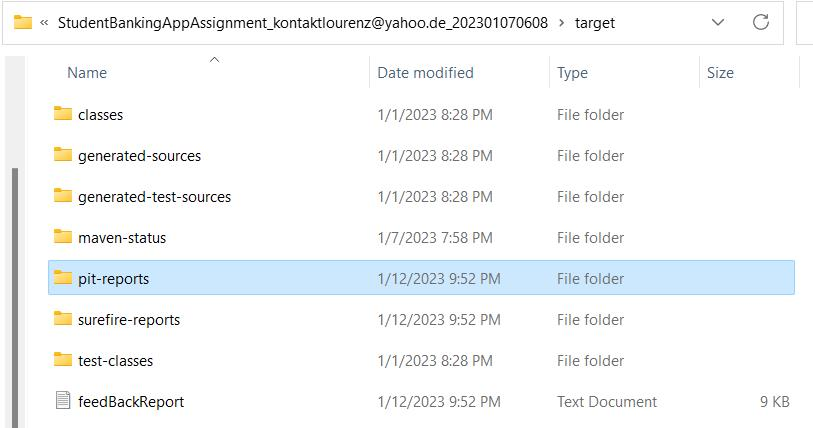
\includegraphics[scale=0.70]{content/fig39.jpg}
	\caption{PiTest report location}
	\label{fig:f11}
\end{figure}

It contains a list of mutation test history folders named in the format year-date-month-hour-mins.\\
Example: 202301071958
\newpage
\begin{figure}[h!]
	\centering
	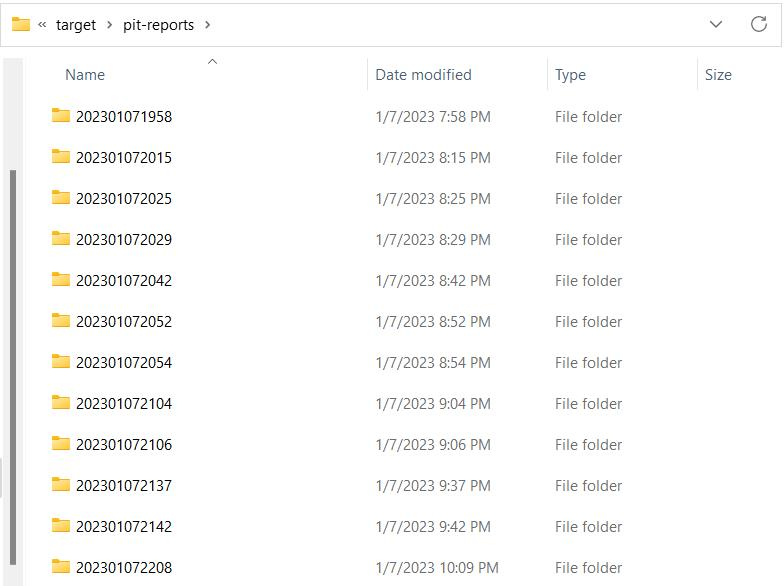
\includegraphics[scale=0.70]{content/fig40.jpg}
	\caption{PiTest report history}
	\label{fig:f11}
\end{figure}
%\newpage
The detail of the PiTest is in the html file.
\begin{figure}[h!]
	\centering
	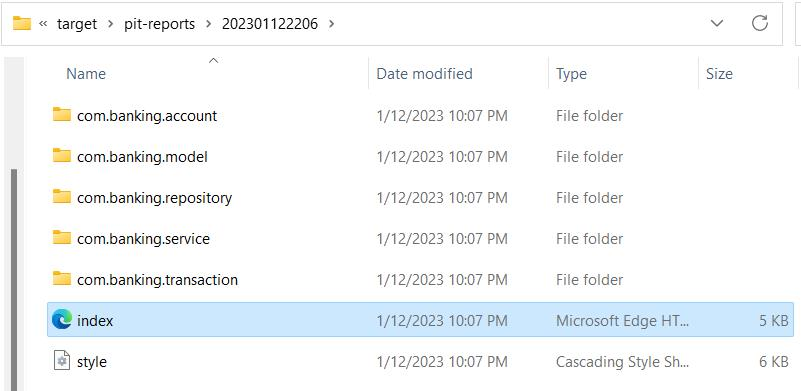
\includegraphics[scale=0.70]{content/fig41.jpg}
	\caption{PiTest report detail location}
	\label{fig:f11}
\end{figure}
\newpage
\begin{figure}[h!]
	\centering
	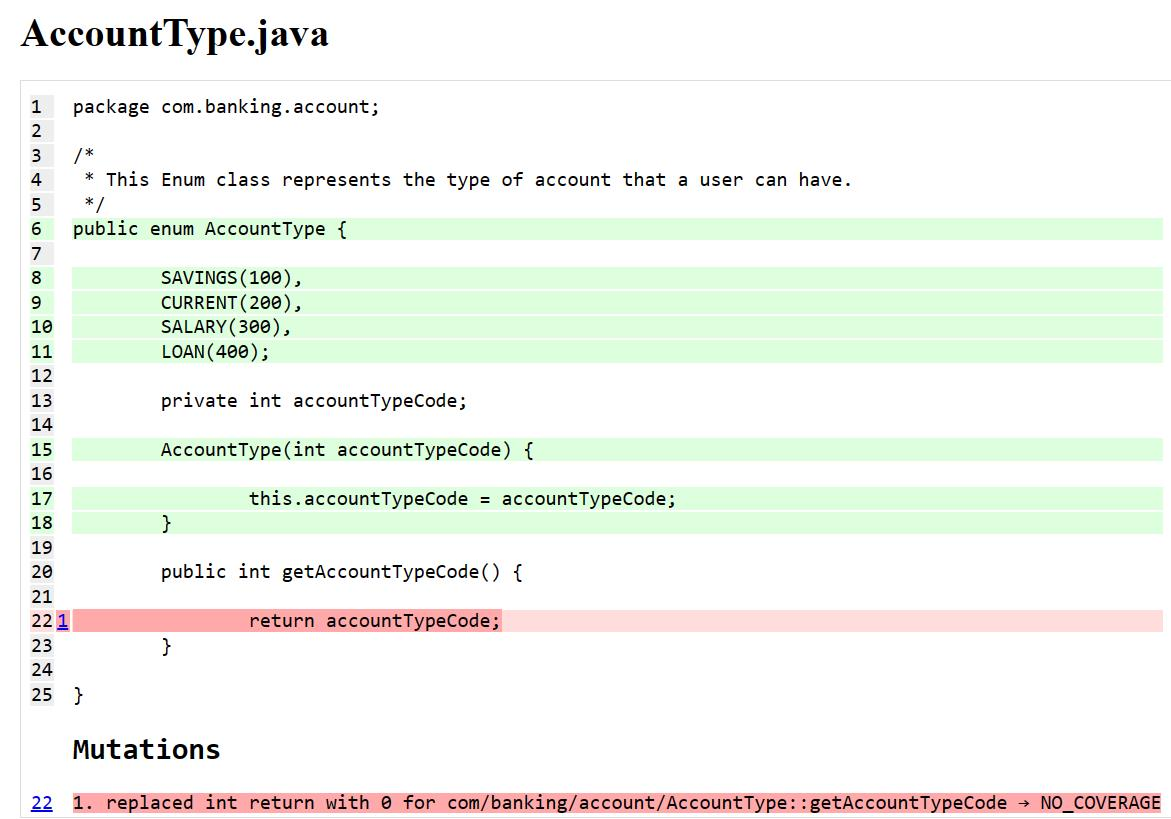
\includegraphics[scale=0.70]{content/fig42.jpg}
	\caption{PiTest report detail}
	\label{fig:f11}
\end{figure}
\newpage
\subsubsection{Feedback message report}
The feedback message report file name “feedBack Report.txt” generated in the folder name “target” of the project being tested.\\
Example: \\%StudentBankingAppAssignment_kontaktlourenz@yahoo.de_202301070608\target\feedBackReport.txt
StudentBankingAppAssignment\_kontaktlourenz@yahoo.de\_202301070608\textbackslash{}target\textbackslash{}feedBackReport.tx
\begin{figure}[h!]
	\centering
	\includegraphics[scale=0.75]{content/fig43.jpg}
	\caption{Feedback report file}
	\label{fig:f11}
\end{figure}

\begin{figure}[h!]
	\centering
	\includegraphics[scale=0.75]{content/fig44.jpg}
	\caption{A part of Feedback report content}
	\label{fig:f11}
\end{figure}



%\noindent\lipsum[10-15]


%\input{mainmatter/chapter-4} % Create file to add

\chapter{EVALUATION}
\label{chapter:EVALUATION}
\section{Overview:}
The purpose of this section is to provide a broad overview of the major findings of the thesis, discuss their importance and answer the research questions raised in Chapter 1. The chapter evaluates and illustrate how the customized feedback system was developed and deployed to provide feedback hints to the students after submitting their JUnit Test solutions on the system. The PiTest is the tool that I used to generate mutants. The outcome of this study have shown that my newly developed customized feedback system was able to effectively provide meaningful and customizable feedback hints to early learners with a basic understanding of JUnit Testing skills. When my customized feedback system is compared to the PiTest feedback system, my feedback system offers better results since its feedback hints explain to the students where they went wrong and how to rectify their mistakes. 

\section{ Evaluation Process}
In this study, 45 students were contacted to participate in the research. Of them, 25 students showed interest to participate in the research while 20 students did not show interest. Of the 25 students that showed interest only 14 of them completed their assignments and submitted their solutions successfully while 11 students failed to submit their solutions. The student participants were provided with assignments of a Java Application named StudentBankingAppAssignment, which was a banking demo application, with functionalities to withdraw money, pay in money and check balance. The students who agreed to participate in the research were required to complete the assignments and submit their solutions to the proposed feedback system. \\
\\
The students were then given more instructions, following which they were to carry out the tasks and submit their solutions. Additionally, I had to provide them instructions of how to name the project, which was provided in a folder that was stored in the drop box. The students were requested to provide a valid email address as the last piece of instruction. Projects processing, Projects failure, Projects Success, Projects Submitted, Projects Incorrect, project assignment was among the folders that could be found in the drop box. After then, the students had two weeks to finish the assignment and submit it via the feedback system. I chose to give the students two weeks so they would have enough time to finish the task, considering that the students may have had other school courses with assignments that they had to complete. \\
\\ 
The students that took part in the evaluation procedure ranged in age from 20 to 27 and were from different universities and colleges but they all belonged to the Computer Science Departments of their respective institutions. According to their feedback, the students who participated volunteered to participate to learn the fundamentals of JUnit testing as well as gain a better understanding of how advanced JUnit testing was carried out in programming assignments while others pointed out that their participation had to do with their passion in programming studies. Some of the students who participated had advanced levels of JUnit testing skills, while others were early learners. The students also had the choice of delivering their work as a Zip file or as a folder containing all the files required to complete their project.\\
\\ 
Students received assistance by being given resources such as tutorial videos explaining to the related assignments, as well as samples of assignment solutions that had passed the basic stage of JUnit testing. This was done to make sure that the students understood what lay ahead of them as far as the assignment is concerned as well as what was expected of them when writing code for their project solutions.  Additionally, the students were supposed to contact a given email address if they had any queries or encounter difficulties in the task they were assigned. The email was meant to be used for requesting help. It's also important to remember that the students that took part in this exercise were from colleges and universities located all over the continents of Africa and Europe.\\
\\
The first step was for the students to access the assignment using a Dropbox folder labeled " project assignment." It is significant to note that not all of the students who were contacted agreed to take part in this evaluation procedure. The solutions to these students' assignments were not entered into the system because they either did not respond when assignments were given to them in the " project assignment" folder or did not follow the instructions that were given to them. While the solutions provided by a different group of students who took part in the assessment were successfully implemented, it was later discovered that these solutions contained errors that prevented the system from processing them further. As a result, these projects were moved into the "projects failure" folder.\\
\\ 
The instructor, myself, determined the root causes of their errors and afterward analyzed the projects that were transferred to the “projects failure” folder in further detail. Another set of students also submitted valid solutions, however, some of these valid solutions did not follow the initial instructions, and as a consequence, they were unable to finish the procedure; as a result, the system transferred them to a folder named "projects incorrect format."\\
\\ 

After the students successfully finished their projects, they had the option of providing their feedback or opinion based on their utilization of the developed feedback system as a whole and how well the assignments were handled. The feedback from the students was mainly positive, as they found that using the proposed feedback system had helped them to understand how advanced JUnit testing was carried out in programming assignments. Many of the students commented on how useful the tutorials and sample solutions had been for giving them an understanding of what was expected when writing code for their own project solutions. Additionally, many of the participants expressed appreciation for being given two weeks to complete their assignments and submit their solutions, as it allowed them enough time to focus on other school coursework while still having enough time to finish their assignments. \\

In terms of negative feedback, some of the participants noted that they would have appreciated more detailed instructions regarding naming conventions for their projects. Others also pointed out that they would have liked more clarification on certain aspects of the assignment such as which libraries were required and what specific types of code snippets were needed for certain functions. Some students also noted that they would have liked more resources available in terms of tutorials or sample solutions. \\

Most of the participants found that using the proposed feedback system was helpful and provided them with a better understanding of how JUnit testing worked in programming assignments. The majority of comments related to issues with instructions or lack of resources, which could be addressed by providing additional guidance or making more resources available online. \\

I evaluated the feedback they provided that was saved in a Dropbox folder called "student feedback opinion." More so this students’ feedback were written in text files. However, it is important to note that the students’ comments and opinions were given anonymously because no personal information regarding the participants was required for this evaluation to avoid data privacy violation. Additionally, the main reason why the feedback was delivered in written text files is just for simplicity’s sake. It was necessary to make it easy for students to provide their feedback of their experience after using the proposed feedback system. \\

% The findings from this research indicate that providing customized feedback may be beneficial for early learners of Object-Oriented Programming as it can help them debug their programs more quickly and easily. Additionally, it provides insight into potential areas of improvement in their solutions, which can help them become better programmers in the long run. Furthermore, utilizing mutation testing tools such as PiTest can help improve the test suites used to evaluate student solutions, leading to more accurate assessment results.\par 
% A customized feedback system aimed at helping students to improve their JUnit testing skills is an important factor in learning. Many tools that offer programming exercises provide automated feedback on student solutions. However, these automated feedbacks do not provide meaningful feedback systems that have solved equations of tests that didn't go through. The system is designed to have features that help classify the feedback hints as something early learners can understand. The techniques used to generate feedback are adaptable and easily evaluated. The system’s time scheduler is advantageous to the students as it helps them set the timers that they prefer. Furthermore, teachers cannot easily adapt schedules of their own as they issue tests to students.\par 
% Given the role of feedback in learning, the development of this customized feedback system wanted to come up with a feedback system that not only helped students with advanced knowledge of JUnit testing but also beginners who had a basic knowledge of JUnit testing skills. The feedback system has narrowed the scope by only considering tools that offer customized feedback hints that let early learners practice by carrying out mutation testing on their own.\par 
% There is a growing body of research on tools for the provision of feedback to students’ assignments the findings of this thesis are that customized feedback is not only limited to early learners but also anyone interested in coding and would like to learn more. Although many feedback systems have been developed, most of them do not include tools that enable students to rectify their mistakes but rather general feedback which might not be helpful for beginner students who only have the basic knowledge. The rationale of my functionality criteria is that the ability to develop a program to solve a particular problem is an important learning objective for learning programming. \par 
% It was discovered that a substantial correlation between the degree to which students engage with the system under test and their impression of the usefulness of the customized feedback system. Another finding was that when assignments are included in the feedback systems curriculum, they effectively play a key role in on how beginner students adapt to programming courses.  
% Since my main interest is to improve learning, I focus on customized feedback. I used the domain criteria to focus my review on programming languages used in the industry or taught at universities. The type of JUnit test that supports this feedback system determines to a large extent how difficult it is to generate feedback. The solutions submitted by the students in the customized feedback system are often quiz-like questions with a single solution, in a program that needs to undergo the who feedback system so that meaningful feedback hints can be sent to the students. During the evaluation stages, students can receive feedback if their solution failed to pass a particular stage. One advantage of this system is that students are allowed to rectify their mistakes and resubmit the solution. Usually a program skeleton or other information that suggests the solution strategy is provided, but variations in the implementation are allowed. I select papers and tools that satisfy all inclusion criteria and none of the exclusion criteria. Since no review addressing my research questions has been conducted before, my customized feedback system has a complete overview of the field.
\section{Importance of the findings}

The data collected from my proposed feedback system with mutation testing shows that it is both simple and provides meaningful feedback. I had carefully categorized and organized the codebase into packages and folders, which made the system easier to use and understand for tutors and professors. Additionally, I used Dropbox to store project files submitted by students, which increased the flexibility of the system. \par

The evaluation process revealed that the student participants responded positively to the system and found it easy to use while providing meaningful feedback. The students felt that they could finish their assignments quickly due to the detailed instructions provided by me as well as the tutorial videos which helped them understand better how JUnit testing was conducted in programming assignments. Furthermore, they also appreciated the fact that they could submit their solutions as a Zip file or folder containing all the files required for their assignment which made it easier for them to complete their tasks. \par

The advantages of using JUnit tests in code were also demonstrated during this evaluation process. Firstly, writing unit tests helps create a robust system capable of responding gracefully to unforeseen events and user errors. Secondly, JUnit tests can help identify coding bugs early in the development process and provide meaningful feedback that helps developers fix these issues quickly and accurately. Thirdly, unit tests can be used for refactoring code, as they will quickly identify any unintended changes that may occur due to design modifications. Finally, JUnit tests provide a layer of documentation for the codebase making it easier for developers to understand the structure and purpose of each component. 
Having a good test coverage also ensures improved quality of software by helping us validate if our application is free of defects and if it is working as per our expectations. Furthermore, it makes the codebase easy to maintain and reusable so anyone can reference them and execute the test cases in the future. \par

Overall, my data shows that my proposed feedback system was indeed simple and provided meaningful feedback which helped students improve their programming skills quickly and accurately. The use of JUnit testing was key in this process as it enabled me to detect bugs early on in the development process and ensured that my system was robust enough to handle unforeseen events or user errors. All these factors combined resulted in meaningful feedback being generated for programming assignments with mutation testing, thus providing a better understanding result when compared to traditional methods such as manual reviews or peer grading systems. \par


\section{Research questions:}
\begin{enumerate}
\item  What type of auto-generated feedback hints is useful for early learners of OOP with basic knowledge of Unit Testing? 
The first research question focused on determining what type of auto-generated feedback hints would be useful for early learners of OOP with basic knowledge of Unit Testing. The results showed that providing customized feedback hints that were made easy for students to understand and tailored to the individual student’s solutions was beneficial for early learners. Furthermore, utilizing mutation testing tools such as PiTest can help improve the test suites used to evaluate student solutions, leading to more accurate assessment results.
\item  How can the proposed feedback system be fully automated to generate meaningful feedback hints to early learners of OOP with basic knowledge of JUnit testing?
The second research question focused on how the proposed feedback system could be fully automated to generate meaningful feedback hints to early learners of OOP with basic knowledge of JUnit testing. The results indicated that the newly developed feedback system was able to effectively provide meaningful and customizable feedback hints to early learners of Object-Oriented Programming. The feedback system was developed using the PiTest mutation testing tool, which enabled the evaluation of the quality of the student’s submissions. Through this system, students were able to submit their solutions and receive clear and concise feedback hints that were much better than what was generated by PiTest alone.
\end{enumerate}
\\
\\
\\
\\
%\section{ Overview: Summary of the results} 
%The results of this study showed that the newly developed feedback system was able to effectively provide meaningful and customizable feedback hints to early learners of Object-Oriented Programming. The feedback system was developed using the PiTest mutation testing tool, which enabled the evaluation of the quality of the student's submissions. Through this system, students were able to submit their solutions and receive clear and concise feedback hints that were much better than what was generated by PiTest alone. Furthermore, the feedback messages were made easy for students to understand and were provided directly to their emails for review.
%\section{Main findings: Report relevant results concisely and objectively, in a logical order}
%I selected a group of students who had a basic understanding of JUnit Testing skills as test subjects and subjected them to this experiment. Each student was provided with JUnit tests which they were required to solve and submit their solutions to the customized feedback system. Upon their submission, the system moved the submitted solutions from the submitted directory to the working directory and then moved on to the next stage till it provided the customized feedback as explained in “Implementation.”
%The findings from this research indicate that providing customized feedback may be beneficial for early learners of Object-Oriented Programming as it can help them debug their programs more quickly and easily. Additionally, it provides insight into potential areas of improvement in their solutions, which can help them become better programmers in the long run. Furthermore, utilizing mutation testing tools such as PiTest can help improve the test suites used to evaluate student solutions, leading to more accurate assessment results.
%\section{Research questions: [What makes customized feedback} better? What benefits early learners? What helps debug programs? What uses mutation testing to improve the test suite?]
%This research investigated what makes customized feedback better for early learners of Object-Oriented Programming. The findings suggest that providing customized feedback can be beneficial for students in several ways. Firstly, it can help students debug their programs more quickly and easily by providing specific hints as to where their solutions may have gone wrong. Additionally, it can provide insight into potential areas of improvement in their solutions, thereby helping them become better programmers in the long run. Finally, by utilizing mutation testing tools such as PiTest to improve the test suites used to evaluate student solutions, more accurate assessment results can be achieved.
%\noindent\lipsum[15-20]


\chapter{Discussion and Future Work}
\label{chapter: Discussion and Future Work}
\section{Summary}
The results of this research indicate that providing customized feedback to early learners of Object-Oriented Programming is beneficial in several ways. Firstly, it can help them identify errors in their code more quickly. Secondly, it provides insight into potential areas of improvement in their solutions, which can help them become better in writing JUint test cases in the long run. Lastly, utilizing mutation testing tools such as PiTest is helpful to analyze the students test suites and to evaluate student solutions, leading to more accurate assessment results.
\section{Interpretations}
Looking at the customized feedback system, the evaluation has shown that giving customized feedback hints to students is important as it helps them identify errors in their code and rectify them. In the first interaction of the system, the PITest tool has come out as an outstanding tool that is compatible with this system because it ensures the quality of the student software testing suite and also efficient in generating mutants. 
\\
\\
Generating feedback is a useful way to point out errors in the students' solutions and emphasizes the importance of mutation testing to programming students. It is therefore a valuable technique, and relatively easy to implement using existing test frameworks. Most tools that use automated testing support the PITest tool, because black-box testing does not require using a specific algorithm.
\\
\\
The only aspect that matters is whether the output meets the requirements of the exercise. However, only giving test-based feedback will not in all cases help a student fix an incorrect program. To help a student improve their JUnit testing skills, the feedback given should explain why the test failed, how the code was supposed to be, and suggestions on how to re-edit the code. Feedback on how to proceed is necessary to both fixing problems and progress toward a solution when the students are facing issues. This type of feedback is mostly seen in the form of error correction feedback hints and much less as hints on task-processing steps as well as program improvements.
\\
\\ 
The findings from this research suggest that providing customizable feedback hints is beneficial for early learners of Object-Oriented Programming because it helps them identify their errors and fix them more quickly and easily. It also provides insight into potential areas for improvement in their solutions. Furthermore, utilizing mutation testing tools such as PiTest can help improve the test suites used to evaluate student solutions and lead to more accurate assessment results. Thus, this type of feedback system could be useful for helping students learn and improve their skills over time. Tests suits that passed mutation testing means they are good. 
\\
\\
The system offers the professor and tutor options to customize the feedback hints using text files format. Using text file format, the professor can specify custom feedback hints and the accepted threshold that the student must obtain to be considered as passed. There is a vast number of studies that identify and classify difficulties and errors that early learners encounter in their learning process. In my case, the customizable feedback hints had better level of feedback satisfaction compared to the Pitest generated feedback. 
\section{Advantages}
The advantages of this study are significant because they suggest that providing meaningful and customizable feedback hints is an effective way to help early learners with basic knowledge of OOP improve their Junit testing skills. This type of system would be especially useful for professors or tutors who are teaching large classes or dealing with a large volume of assignments regularly and due to its automated nature, which reduces the amount of time spent giving individualized feedback for each student's assignment solution.
\\
\\
Many of the previous feedback systems have only been able to deliver generalized feedback. However, my customized feedback system goes further to allowing the professor or tutor give a customized feedback hint that early learners with basic knowledge JUnit testing skills can understand. If students want to learn from their mistakes, they should familiarize themselves with using my feedback system. The use of this system enables lecturers to focus their attention to the students whose code failed. By doing so they can engage the students in person and help them identify their weaknesses and improve on them.
\section{Limitations}

The evaluation process used in this study is subject to several limitations that threaten its validity. The first issue relates to the accuracy and meaningfulness of the variables being measured. In this study, the feedback system was tested on a small sample size of 45 students, 25 of whom agreed to participate. This limited sample size may not accurately represent the wider population, as it is impossible to guarantee that the participants were representative of the wider student population in terms of age, experience level and other factors. Furthermore, the assignment given to the participants was relatively simple and straightforward; thus, there may be no way to extrapolate any findings from this evaluation process to more complex programming assignments. \par

Another issue is whether or not any changes observed in performance are attributable solely to the feedback system. As mentioned before, some students failed to submit solutions due to a lack of understanding or technical difficulties; such factors could have had an impact on their performance and should be accounted for when analyzing results. Additionally, the instructor's involvement in providing resources such as tutorial videos and sample solutions could have inadvertently influenced the students’ performance; thus, it would be advisable for future research projects to look into different approaches for providing assistance without having an effect on student performance. \par

Finally, the last limitation deals with how generalizable results from this study are for similar studies in different contexts. The participants in this study were from universities located all over Europe and Africa, so it would be difficult to draw conclusions from this study about how well a similar feedback system would perform at institutions located elsewhere. Furthermore, as noted earlier, some students found certain aspects of the assignment difficult or overly time-consuming; thus, any conclusions drawn from this study may not apply when dealing with more complex assignments at other institutions. \par

In conclusion, while this evaluation process has provided valuable insights into how well a feedback system can improve student programming performance through mutation testing techniques, further research is necessary before these findings can be generalized across different contexts.


\section{Conclusion}
The research on feedback systems has demonstrated that providing relevant and customizable feedback hints is a successful strategy for assisting early learners in learning and improving their JUnit testing skills over time. The evaluation showed that the structure of the customizable feedback hints was simple, which enabled the students to understand it easily. This implies that the system will so be great for lecturers who have to deal with a large number of students assignments. Although early learners are the target group, the system can also generate feedback for more experienced programmers because the feedback hints are customizable. \par

The feedback system was organized into categories and arranged into basic folders for easy understanding and scalability. Descriptive class and method names were used to enable the readability of the source code by other Java developers. This approach facilitates future expansions while ensuring clarity of the system design. \par

Tracking activity of students using the system revealed that those who got regular feedback hints submitted more solutions than those who did not get any hints. In addition, a comparison between the time taken by feedback systems and manual feedback showed a significant difference in favor of automated evaluation and giving of feedback. The data gathered from my feedback system suggests that it is indeed simple and provides meaningful feedback hints that aid students in improving their programming skills quickly. Furthermore, the feedback hints are customizable, making the system even more effective in helping students reach their desired proficiency level. \par

In conclusion, this research has demonstrated that providing relevant and customizable feedback hints is an effective strategy for assisting early learners in learning and improving their JUnit testing skills over time. The development of feedback systems opened the door for significant programming improvements in the way JUnit testing concepts were presented to early learners of OOP and how the customized feedback hints assisted them in sharpening their skills. \par

The use of feedback systems is generally perceived to be excellent in giving customized hints on JUnit tests; however, further research should look more closely at how historical information about student solutions may be used to enhance such suggestions as well as explore new technologies and designs used for creating future automated evaluation systems with multiple feedback hints per mutation testing process.

\section{Future Work}
Based on these findings, it is recommended that further analyses could be conducted on how automated feedback systems affect students at different levels or with different types of programming backgrounds before any definitive conclusions can be drawn about its effectiveness overall across all types of programming courses or assignments. I have tried to locate as many various references that will support my arguments as feasible to make my system as dependable as possible. My thesis' credibility is founded on present knowledge and actuality.\\
\\
 Additionally, future work shall involve adding a user interface so that the professor does not influence the feedback hints by adjusting the customizable feedback hints and thresholds more easily. The system shall also generate feedback hints that are auto-edited instead of having the professor pre-written on text files which is tiresome and time-consuming. 
% The results of this research indicate that providing customized feedback to early learners of Object-Oriented Programming is beneficial in several ways. Firstly, it can help them identify errors in their code programs more quickly and easily by providing customized feedback hints as to where their solutions may have gone wrong. Secondly, it provides insight into potential areas of improvement in their solutions, which can help them become better programmers in the long run. Lastly, utilizing mutation testing tools such as PiTest can help improve the test suites used to evaluate student solutions, leading to more accurate assessment results.
% \section{Interpretations}
% Looking at the customized feedback system, the results have shown that giving customized feedback to students is important as it helps the identify errors in a code and rectify them. In the first interaction of the system, the PITest tool has come out as an outstanding tool that is compatible with this system and it is accurate and efficient in generating mutants. Generating feedback based on tests is a useful way to point out errors in student solutions and emphasizes the importance of mutation testing to programming students. It is therefore a valuable technique, and relatively easy to implement using existing test frameworks. Most tools that use automated testing support the PITest tool, because black-box testing does not require using a specific algorithm.\par 
% The only aspect that matters is whether the output meets the requirements of the exercise. However, only giving test-based feedback will not in all cases help a student fix an incorrect program. To help a student improve their JUnit testing skills, the feedback given should explain why the test failed, how the code was supposed to be, and suggestions on how to re-edit the code. Feedback on how to proceed is necessary to both fix problems and progress toward a solution when stuck. This type of feedback is mostly seen in the form of error correction feedback hints and much less as hints on task-processing steps as well as program improvements.\par 
% The findings from this research suggest that providing customized feedback is beneficial for early learners of Object-Oriented Programming because it helps them identify their errors and fix them more quickly and easily and provides insight into potential areas for improvement in their solutions. Furthermore, utilizing mutation testing tools such as PiTest can help improve the test suites used to evaluate student solutions and lead to more accurate assessment results. Thus, this type of feedback system could be useful for helping students learn and grow as programmers over time.\par 
%  Tests suits that passed mutation testing means they are good and accurate. The correct test suites can be obtained and applied to programming and work precisely while delivering accurate and efficient results. In dynamic analysis, they are used for running test cases to generate the expected output. In static analysis, the structure of a correct solution is compared to the structure of a student solution. To recognize more than one solution variant, the PITest tool accepts multiple solutions that each represent a different algorithm to solve the problem. This enables multiple feedback to be given to students within a short time duration.\par 
% The system offers the professor several options to customize the hints using special commands embedded in the comments. Using these commands the professor can specify custom hint messages and control which parts of the code should be revealed or not. The system includes a default revealing mechanism that shows the basic structure of the code and ends at the level that shows all code.\par 
% There is a vast amount of studies that identify and classify difficulties and errors that novice programmers encounter in their learning process. In my case, the customized feedback system had higher levels of feedback satisfaction compared to generalized feedback. This study is also crucial in assessing the effectiveness of customized feedback in terms of both academic achievement and satisfaction with feedback compared to generalized feedback.
% \section{Implications}
% The implications of this study are significant because they suggest that providing meaningful and customizable feedback hints is an effective way to help beginners learn and develop programming skills over time with greater ease and accuracy. This type of system would be especially useful for instructors or tutors who are teaching large classes or dealing with a large volume of assignments regularly due to its automated nature which reduces the amount of time spent giving individualized feedback for each student's assignment solution.\par 
% Many of the previous feedback systems have only been able to deliver generalized feedback. However, my customized feedback system goes further to give a customized feedback hint that beginner students with basic JUnit testing skills can understand. If students want to learn from their mistakes, they should familiarize themselves with using my customized feedback system. The use of this system enables lecturers to turn their attention to the students whose code failed. By doing so they can engage the students physically and help them identify their mistakes and improve.
% \section{Limitations}
% Despite the promising findings from this study, some limitations should be noted when interpreting these results. It was discovered that customized feedback did not improve students' academic achievement, despite the precedence set by the literature. However, it was discovered that the students who received customized feedback expressed feedback satisfaction at much greater levels.
% Additionally, this study did not investigate whether or not this type of automated feedback system had any potential negative impact on student learning outcomes; thus further research should also be conducted to assess any potential drawbacks associated with using automated systems like these before they are widely implemented in classrooms or other educational settings around the world.\par 
%  Some students believed that the exercise's improper parametrization made it difficult to compute the system's inputs. Additionally, others thought that the task required laborious, mechanical processes that diminished the learning process and frequently resulted in dissatisfaction. I appreciate the validity of these critiques and admit that much more effort has to be done to improve both the content and presentation of future assignments in the customized feedback because this is the first actual deployment and testing of the customized feedback. 
% \section{Recommendations and future studies}
% Based on these findings, it is recommended that further studies or analyses be conducted on how automated feedback systems like these affect students at different levels or with different types of programming backgrounds before any definitive conclusions can be drawn about its effectiveness overall across all types of programming courses or assignments. I have tried to locate as many various references that will support my arguments as feasible to make my system as dependable as possible. My thesis' credibility is founded on present knowledge and actuality.\par 
%  Additionally, future work shall involve adding a user interface so that the professor does not influence the feedback hints by adjusting their thresholds therefore, the hits should entirely be auto-generated to deliver meaningful feedback to the students especially beginner students with basic knowledge. The system shall also generate feedback hints that are auto-edited instead of having the professor edit them manually which is tiresome and time-consuming. Although the resulting feedback hits might seem robotic rather than manual because of limited human intervention, the system shall been customized to deliver feedback hits that will be as good as manual.\par 
% The diversity of feedback types has increased over the last decades and new techniques are being applied to generate feedback that is increasingly helpful for students. Therefore, if a similar study were to be conducted at a different time, it's feasible that the results would be different. Given that my thesis deals with customized feedback, a relatively new concept, significant modifications may be made in one or more of these fields.
% The most frequent types of feedback are still test failures and solving problems when taking into account past data. The diversity of feedback styles has, however, grown in the twenty-first century, which is a good thing.

%\section{Summary: Recap of key results}
%The results of this research indicate that providing customized feedback to early learners of Object-Oriented Programming is beneficial in several ways. Firstly, it can help them debug their programs more quickly and easily by providing specific hints as to where their solutions may have gone wrong. Secondly, it provides insight into potential areas of improvement in their solutions, which can help them become better programmers in the long run. Lastly, utilizing mutation testing tools such as PiTest can help improve the test suites used to evaluate student solutions, leading to more accurate assessment results.
%\section{Interpretations: Meaning behind the results}
%The findings from this research suggest that providing customized feedback is beneficial for early learners of Object-Oriented Programming because it helps them debug their programs more quickly and easily and provides insight into potential areas for improvement in their solutions. Furthermore, utilizing mutation testing tools such as PiTest can help improve the test suites used to evaluate student solutions and lead to more accurate assessment results. Thus, this type of feedback system could be useful for helping students learn and grow as programmers over time. 
%\section{Implications: Significance of the results}
%The implications of this study are significant because they suggest that providing meaningful and customizable feedback hints is an effective way to help beginners learn and develop programming skills over time with greater ease and accuracy. This type of system would be especially useful for instructors or tutors who are teaching large classes or dealing with a large volume of assignments regularly due to its automated nature which reduces the amount of time spent giving individualized feedback for each student's assignment solution.
%\section{Limitations: What cannot be deduced from the results?}
%Despite the promising findings from this study, some limitations should be noted when interpreting these results. Firstly, this study only focused on early learners with basic knowledge of JUnit testing; thus further research should be conducted on how this type of feedback system affects students at different levels or with different types of programming backgrounds before any definitive conclusions can be drawn about its effectiveness overall across all types of programming courses or assignments. Additionally, this study did not investigate whether or not this type of automated feedback system had any potential negative impact on student learning outcomes; thus further research should also be conducted to assess any potential drawbacks associated with using automated systems like these before they are widely implemented in classrooms or other educational settings around the world.  
%\section{Recommendations: Further studies or analyses}
%Based on these findings, it is recommended that further studies or analyses be conducted on how automated feedback systems like these affect students at different levels or with different types of programming backgrounds before any definitive conclusions can be drawn about its effectiveness overall across all types of programming courses or assignments. Additionally, further research should also be conducted to assess any potential drawbacks associated with using automated systems like these before they are widely implemented in classrooms or other educational settings around the world. Finally, further research should also be conducted on how to optimize the feedback provided by these systems to maximize their effectiveness in helping students learn and develop programming skills over time.

%\chapter{Conclusion}
\label{chapter:conclusion}



% \newpage
% \setcounter{secnumdepth}{-1}
%\section*{Acknowledgement} % * title not in table of contents
I want to thank AA, who served as my primary supervisor, for guiding me through this project. Secondly, I want to express my gratitude to my friends and family for their encouragement and insightful comments on the study.\par 
I want to thank the Free University of Berlin's Economics department's technical and support personnel for their assistance. I also want to express my sincere gratitude to my supervisors, who assisted me in completing my assignment.


% % some example sentences you could use for the acknowledgement
% First, I like to thank my first supervisor .... , for .... . Also, I want to thank my second supervisor .... for .... .\\

% \noindent
% Thanks to ..... for all the insights into .... . Thanks to .... for all the intense but fruitful scientific debate about .... . Thanks to ... , who always had an open door for ..... . \\

% \noindent
% Also, I would like to thank the .... . \newline

% \noindent
% And last but not least, thanks to .... , who helped ..... . As well as .... for the help with .... . 

%% Prevent urls running into margins in bibliography
\setcounter{biburlnumpenalty}{7000}
\setcounter{biburllcpenalty}{7000}
\setcounter{biburlucpenalty}{7000}



%%  Add the bibliography
\printbibliography[title = {References}]



% Letters for chapters
\appendix

% \newpage
% \setcounter{secnumdepth}{-1}

%%\chapter*{Eidesstattliche Versicherung}

Hiermit versichere ich an Eides statt, dass ich die vorliegende Arbeit im Studiengang ......... selbstständig verfasst und keine anderen als die angegebenen Hilfsmittel – insbesondere keine im Quellenverzeichnis nicht benannten Internet-Quellen – benutzt habe. Alle Stellen, die wörtlich oder sinngemäß aus Veröffentlichungen entnommen wurden, sind als solche kenntlich gemacht. Ich versichere weiterhin, dass ich die Arbeit vorher nicht in einem anderen Prüfungsverfahren eingereicht habe und die eingereichte schriftliche Fassung der auf dem elektronischen Speichermedium entspricht.\newline

\noindent
Einer Veröffentlichung der vorliegenden Arbeit in der zuständigen Fachbibliothek des Fachbereichs stimme ich zu.\newline


\vspace{25mm}

%  The aligning options are m for middle, p for top and b for bottom. 
\noindent
\begin{tabular}{@{}p{2.5cm}p{3cm}p{2cm}p{7cm}}
Hamburg, den  & \hrulefill & Unterschrift: & \hrulefill \\
\end{tabular}


  



\begin{comment}
    Bei der Abgabe der Abschlussarbeit ist eine Versicherung an Eides statt (lt. § 59 Abs. 3 HmbHG) abzugeben:

„Hiermit versichere ich an Eides statt, dass ich die vorliegende Arbeit im Studiengang ...*) selbstständig verfasst und keine anderen als die angegebenen Hilfsmittel – insbesondere keine im Quellenverzeichnis nicht benannten Internet-Quellen – benutzt habe. Alle Stellen, die wörtlich oder sinngemäß aus Veröffentlichungen entnommen wurden, sind als solche kenntlich gemacht. Ich versichere weiterhin, dass ich die Arbeit vorher nicht in einem anderen Prüfungsverfahren eingereicht habe und die eingereichte schriftliche Fassung der auf dem elektronischen Speichermedium entspricht.“             *) bitte Ihren Studiengang und Abschluss eintragen

Die Angabe zur Veröffentlichung in der Fachbibliothek können Sie direkt in die Versicherung mit einbeziehen:

"Einer Veröffentlichung der vorliegenden Arbeit in der zuständigen Fachbibliothek des Fachbereichs stimme ich zu/stimme ich nicht zu."

Bitte drucken Sie diese Versicherung in jedem Exemplar am Ende ab und unterschreiben Sie diese mit der Angabe von Ort und Datum.
\end{comment}





%\input{appendix/appendix-a}





\end{document}